\documentclass[compress]{beamer}
\usepackage{ifthen,verbatim}

\newcommand{\isnote}{}
\xdefinecolor{lightyellow}{rgb}{1.,1.,0.25}
\xdefinecolor{darkblue}{rgb}{0.1,0.1,0.7}

%% Uncomment this to get annotations
%% \def\notes{\addtocounter{page}{-1}
%%            \renewcommand{\isnote}{*}
%% 	   \beamertemplateshadingbackground{lightyellow}{white}
%%            \begin{frame}
%%            \frametitle{Notes for the previous page (page \insertpagenumber)}
%%            \itemize}
%% \def\endnotes{\enditemize
%% 	      \end{frame}
%%               \beamertemplateshadingbackground{white}{white}
%%               \renewcommand{\isnote}{}}

%% Uncomment this to not get annotations
\def\notes{\comment}
\def\endnotes{\endcomment}

\setbeamertemplate{navigation symbols}{}
\setbeamertemplate{headline}{\mbox{ } \hfill
\begin{minipage}{5.5 cm}
\vspace{-0.75 cm} \small
\end{minipage} \hfill
\begin{minipage}{4.5 cm}
\vspace{-0.75 cm} \small
\begin{flushright}
\ifthenelse{\equal{\insertpagenumber}{1}}{}{Jim Pivarski \hspace{0.2 cm} \insertpagenumber\isnote/\pageref{numpages}}
\end{flushright}
\end{minipage}\mbox{\hspace{0.2 cm}}\includegraphics[height=1 cm]{../cmslogo} \hspace{0.1 cm} \includegraphics[height=1 cm]{../tamulogo} \hspace{0.01 cm} \vspace{-1.05 cm}}

\begin{document}
\begin{frame}
\vfill
\begin{center}
\textcolor{darkblue}{\Large Effect of DT Internal Alignment on Sawtooth}

\vfill
\begin{columns}
\column{0.3\linewidth}
\begin{center}
\large
\textcolor{darkblue}{Jim Pivarski}
\end{center}
\end{columns}

\begin{columns}
\column{0.3\linewidth}
\begin{center}
\scriptsize
{\it Texas A\&M University}
\end{center}
\end{columns}

\vfill
18 May, 2009

\end{center}
\end{frame}

%% \begin{notes}
%% \item This is the annotated version of my talk.
%% \item If you want the version that I am presenting, download the one
%% labeled ``slides'' on Indico (or just ignore these yellow pages).
%% \item The annotated version is provided for extra detail and a written
%% record of comments that I intend to make orally.
%% \item Yellow notes refer to the content on the {\it previous} page.
%% \item All other slides are identical for the two versions.
%% \end{notes}

\small

\begin{frame}
\frametitle{New alignment must have}

\begin{itemize}
\item Latest tracker alignment and APEs (alignment already exists, APEs will be ready in a few days) \textcolor{darkblue}{(not included here)}
\item Latest magnetic field (no developments more recent than a few weeks ago)
\item New internal DT alignment, if that is accepted
\item High $p_T$ (100--200~GeV, see last muon POG)
\item CMSSW\_2\_2\_11
\end{itemize}

\vfill
\hspace{-0.83 cm} \textcolor{darkblue}{\Large This talk shows a HIP global alignment with the new internal DT alignment, with a focus on the sawtooth effect in residuals}
\end{frame}

\begin{frame}
\frametitle{Iteration-by-iteration changes}

\begin{itemize}
\item Aligning $x$, $y$, $\phi_x$, $\phi_y$, $\phi_z$ in stations 1--3, wheel 0
\item Aligning $x$, $\phi_x$, $\phi_y$, $\phi_z$ in stations 1--3, other wheels
\item Aligning $x$, $\phi_y$, $\phi_z$ in station 4
\end{itemize}

\vfill
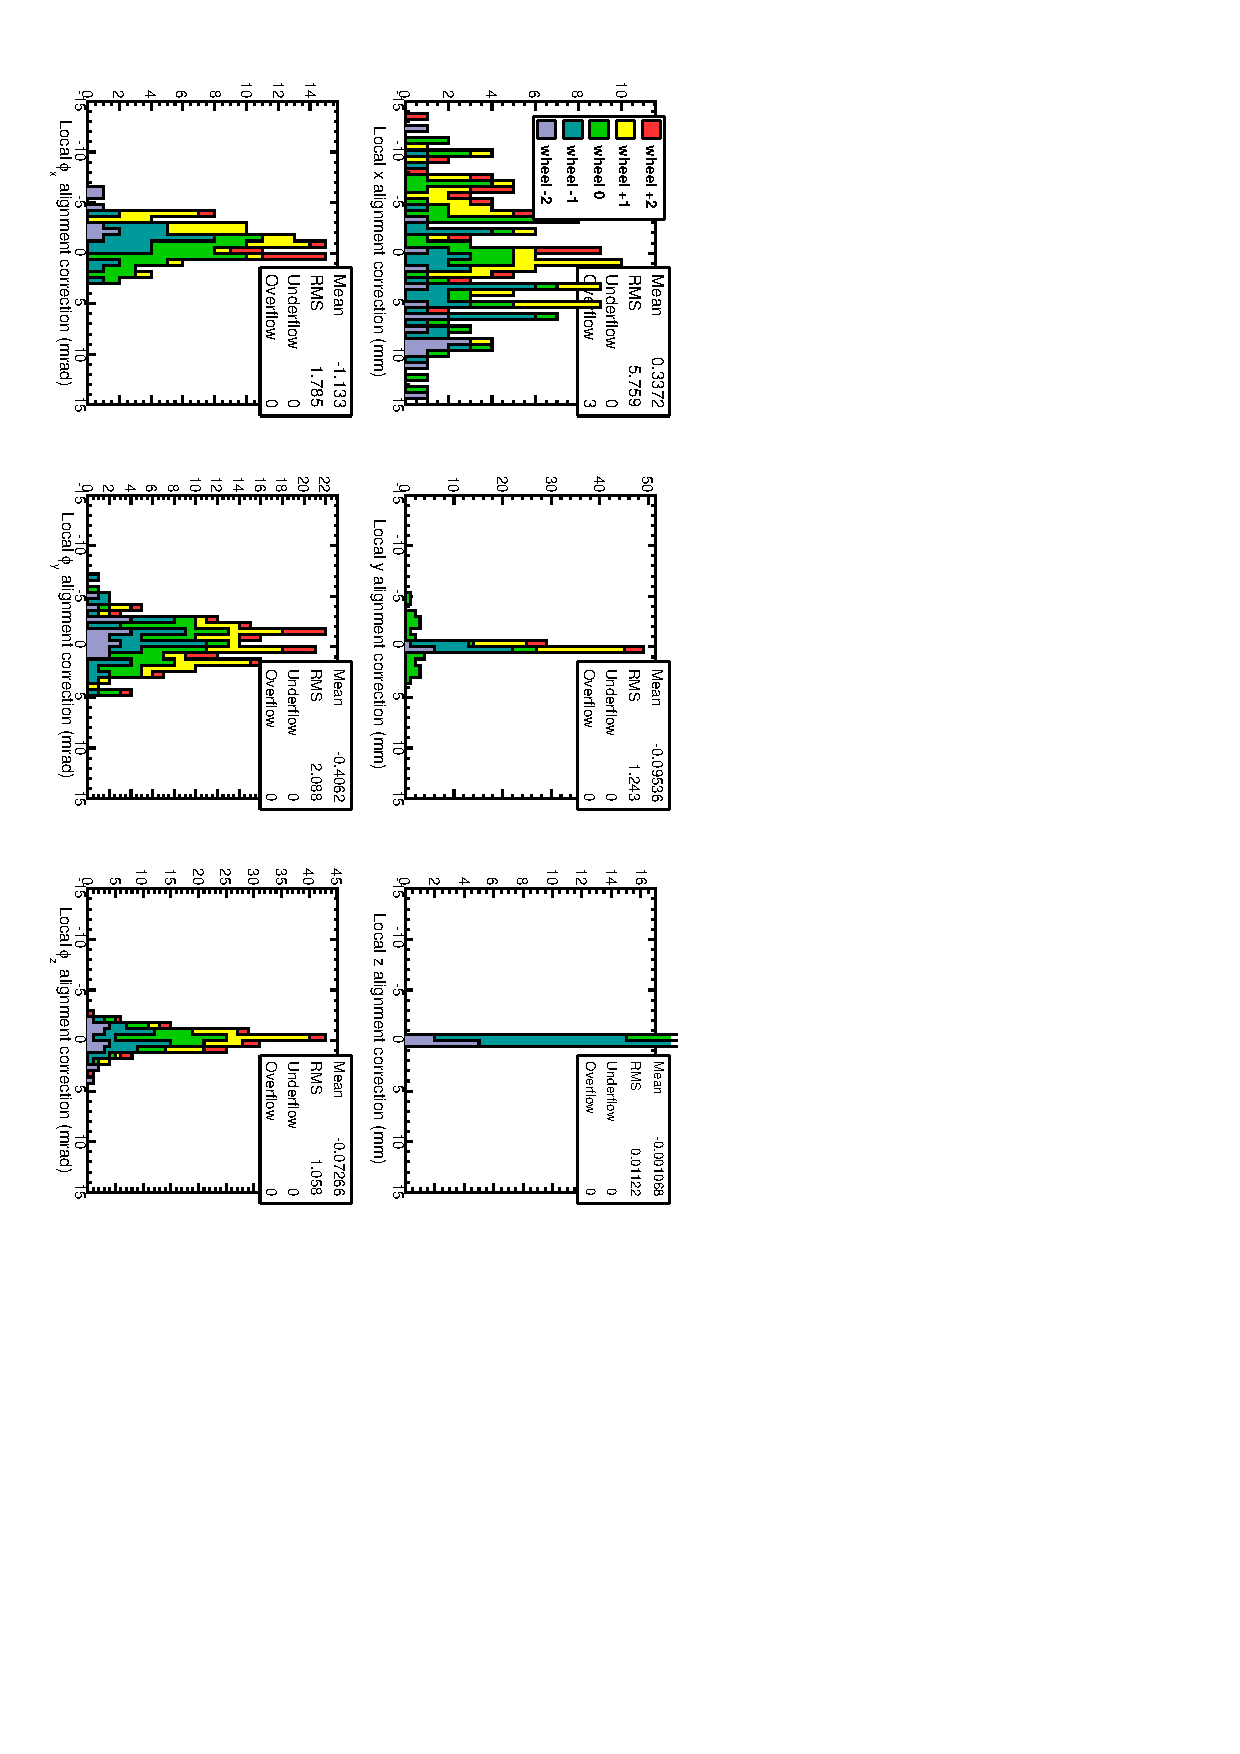
\includegraphics[height=\linewidth, angle=90]{data_100GeV_newinternal_iter1.pdf}
\end{frame}

\begin{frame}
\frametitle{Iteration-by-iteration changes}

\begin{itemize}
\item Aligning $x$, $y$, $\phi_x$, $\phi_y$, $\phi_z$ in stations 1--3, wheel 0
\item Aligning $x$, $\phi_x$, $\phi_y$, $\phi_z$ in stations 1--3, other wheels
\item Aligning $x$, $\phi_y$, $\phi_z$ in station 4
\end{itemize}

\vfill
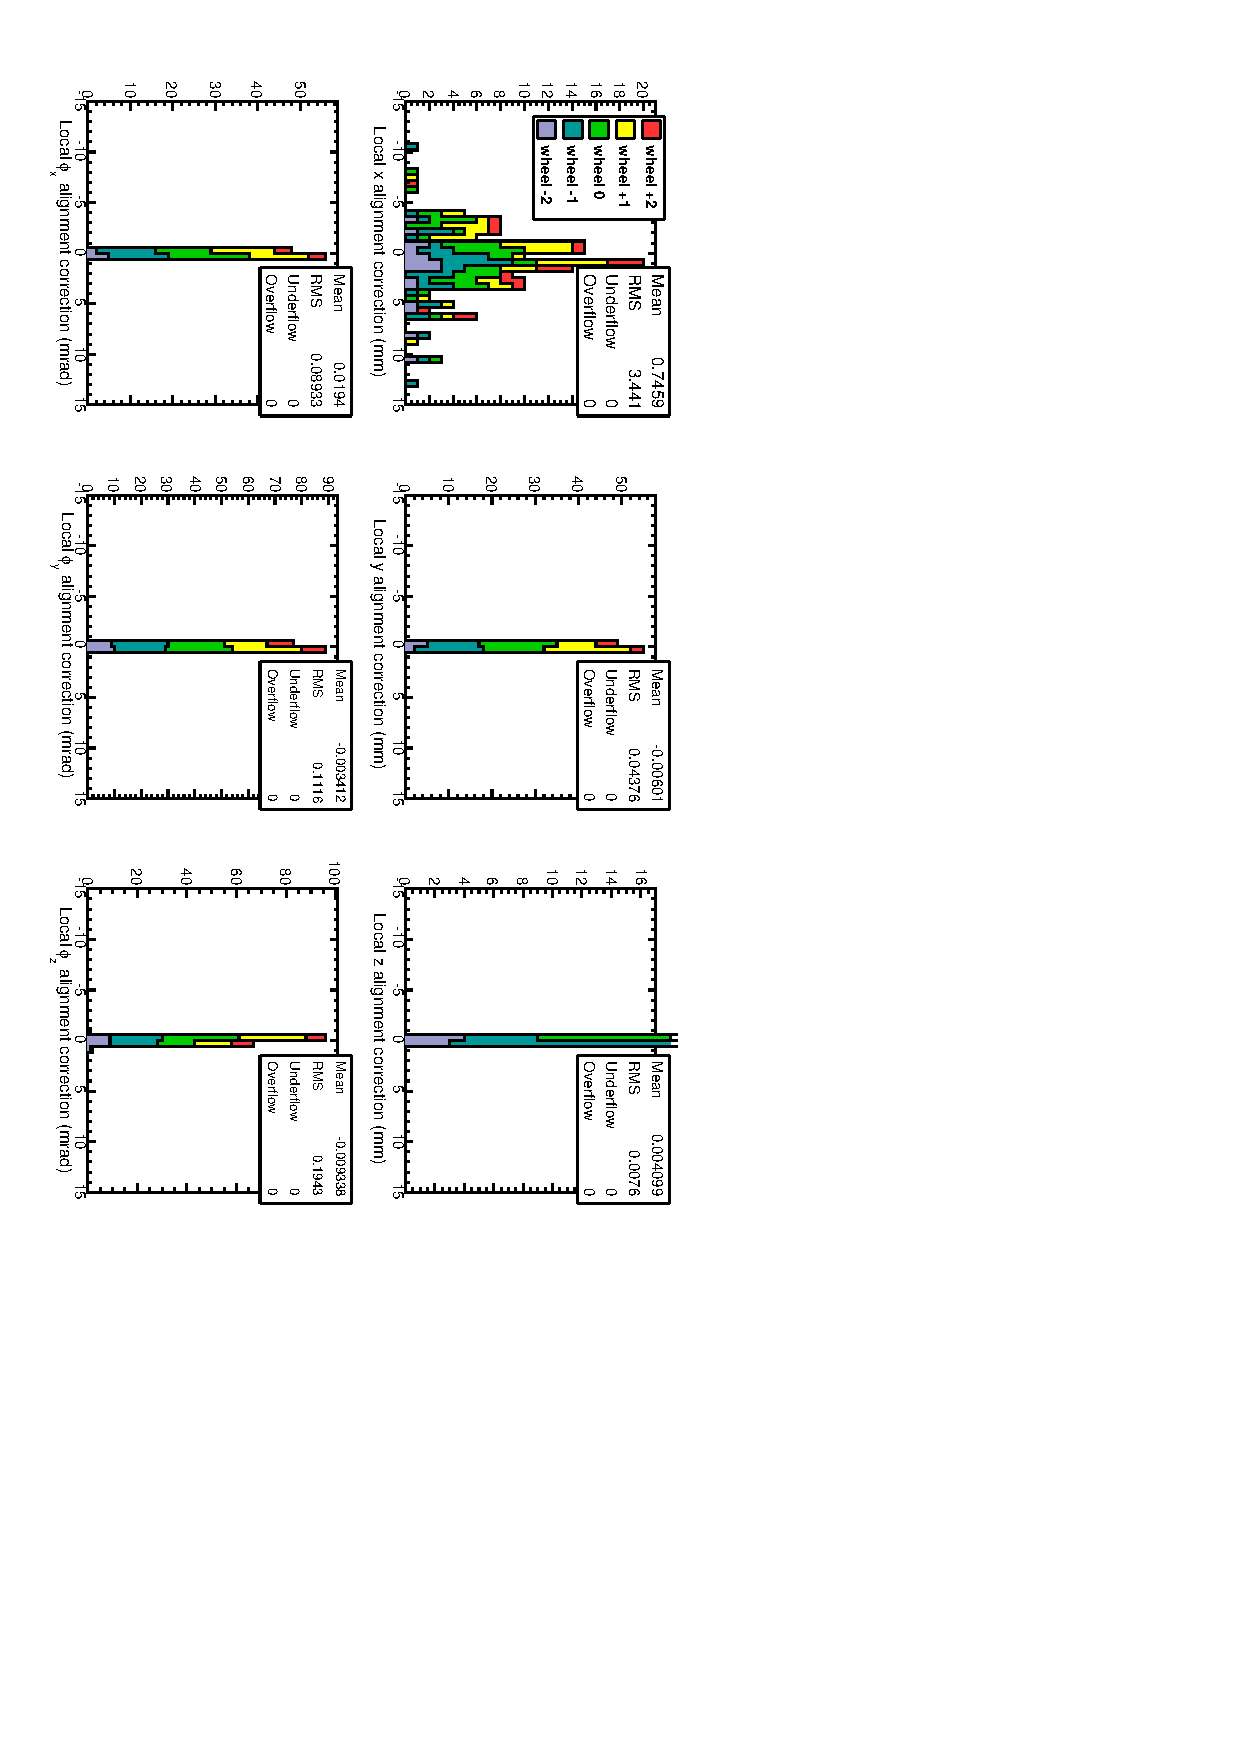
\includegraphics[height=\linewidth, angle=90]{data_100GeV_newinternal_iter2.pdf}
\end{frame}

\begin{frame}
\frametitle{Iteration-by-iteration changes}

\begin{itemize}
\item Aligning $x$, $y$, $z$, $\phi_x$, $\phi_y$, $\phi_z$ in stations 1--3, wheel 0
\item Aligning $x$, $y$, $z$, $\phi_x$, $\phi_y$, $\phi_z$ in stations 1--3, other wheels
\item Aligning $x$, $\phi_y$, $\phi_z$ in station 4
\end{itemize}

\vfill
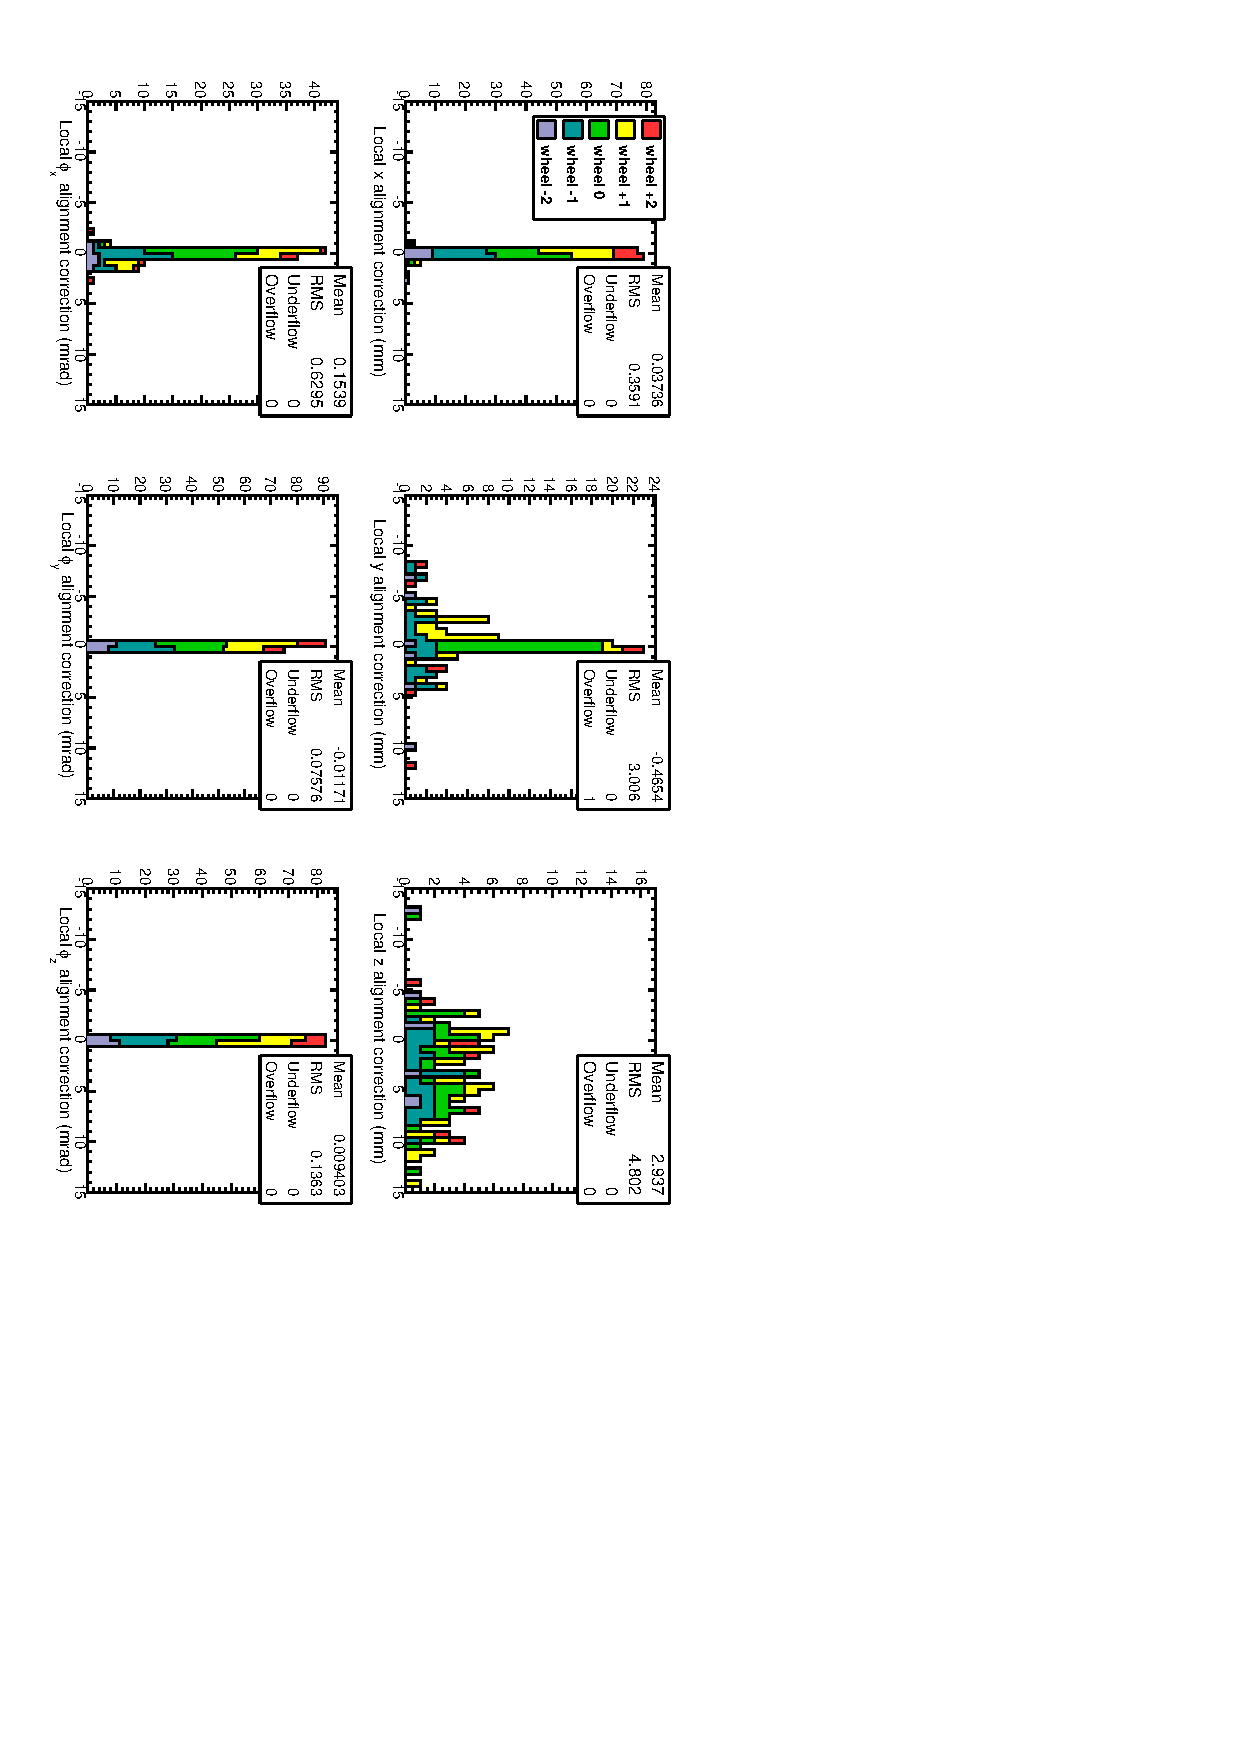
\includegraphics[height=\linewidth, angle=90]{data_100GeV_newinternal_iter3.pdf}
\end{frame}

\begin{frame}
\frametitle{Iteration-by-iteration changes}

\begin{itemize}
\item Aligning $x$, $y$, $z$, $\phi_x$, $\phi_y$, $\phi_z$ in stations 1--3, wheel 0
\item Aligning $x$, $y$, $z$, $\phi_x$, $\phi_y$, $\phi_z$ in stations 1--3, other wheels
\item Aligning $x$, $\phi_y$, $\phi_z$ in station 4
\end{itemize}

\vfill
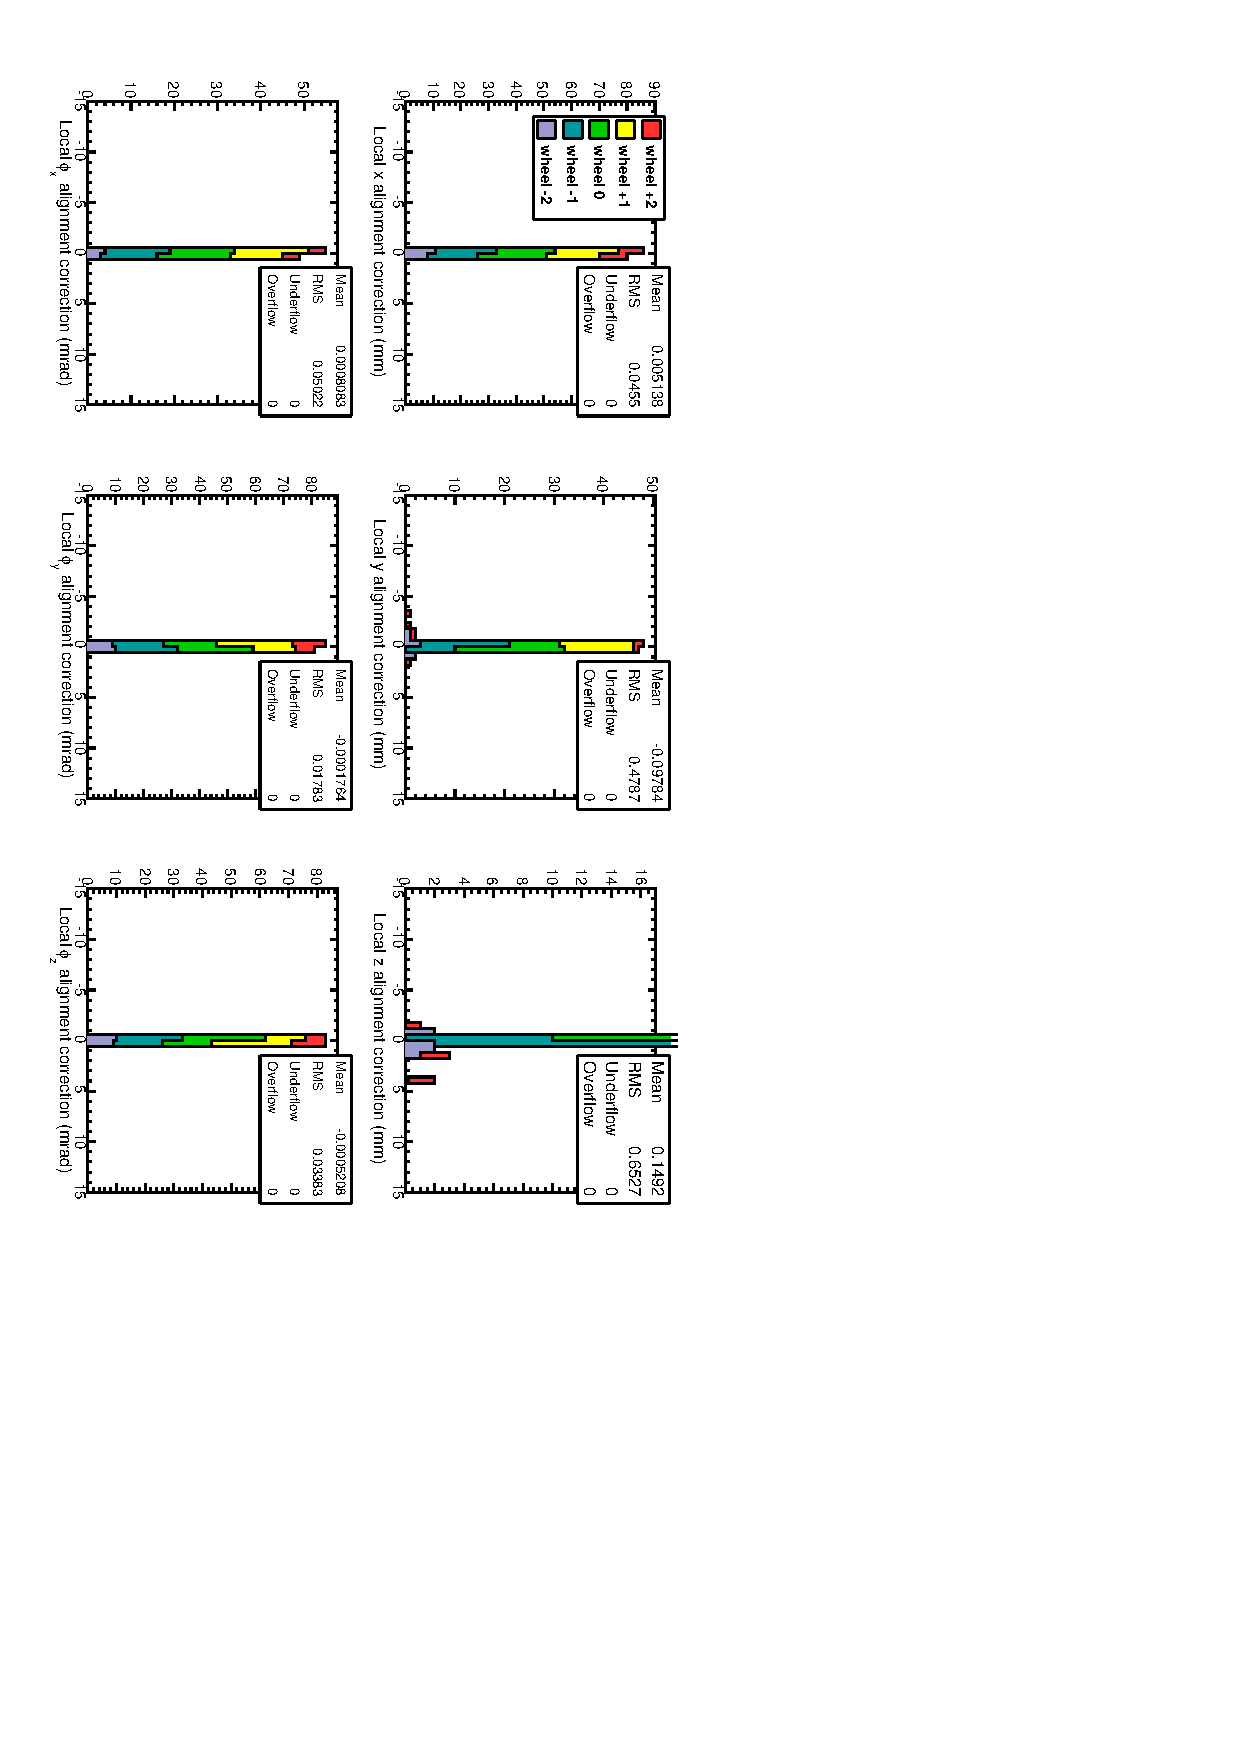
\includegraphics[height=\linewidth, angle=90]{data_100GeV_newinternal_iter4.pdf}
\end{frame}

\begin{frame}
\frametitle{Iteration-by-iteration changes}

\begin{itemize}
\item Aligning $x$, $y$, $z$, $\phi_x$, $\phi_y$, $\phi_z$ in stations 1--3, wheel 0
\item Aligning $x$, $y$, $z$, $\phi_x$, $\phi_y$, $\phi_z$ in stations 1--3, other wheels
\item Aligning $x$, $\phi_y$, $\phi_z$ in station 4
\end{itemize}

\vfill
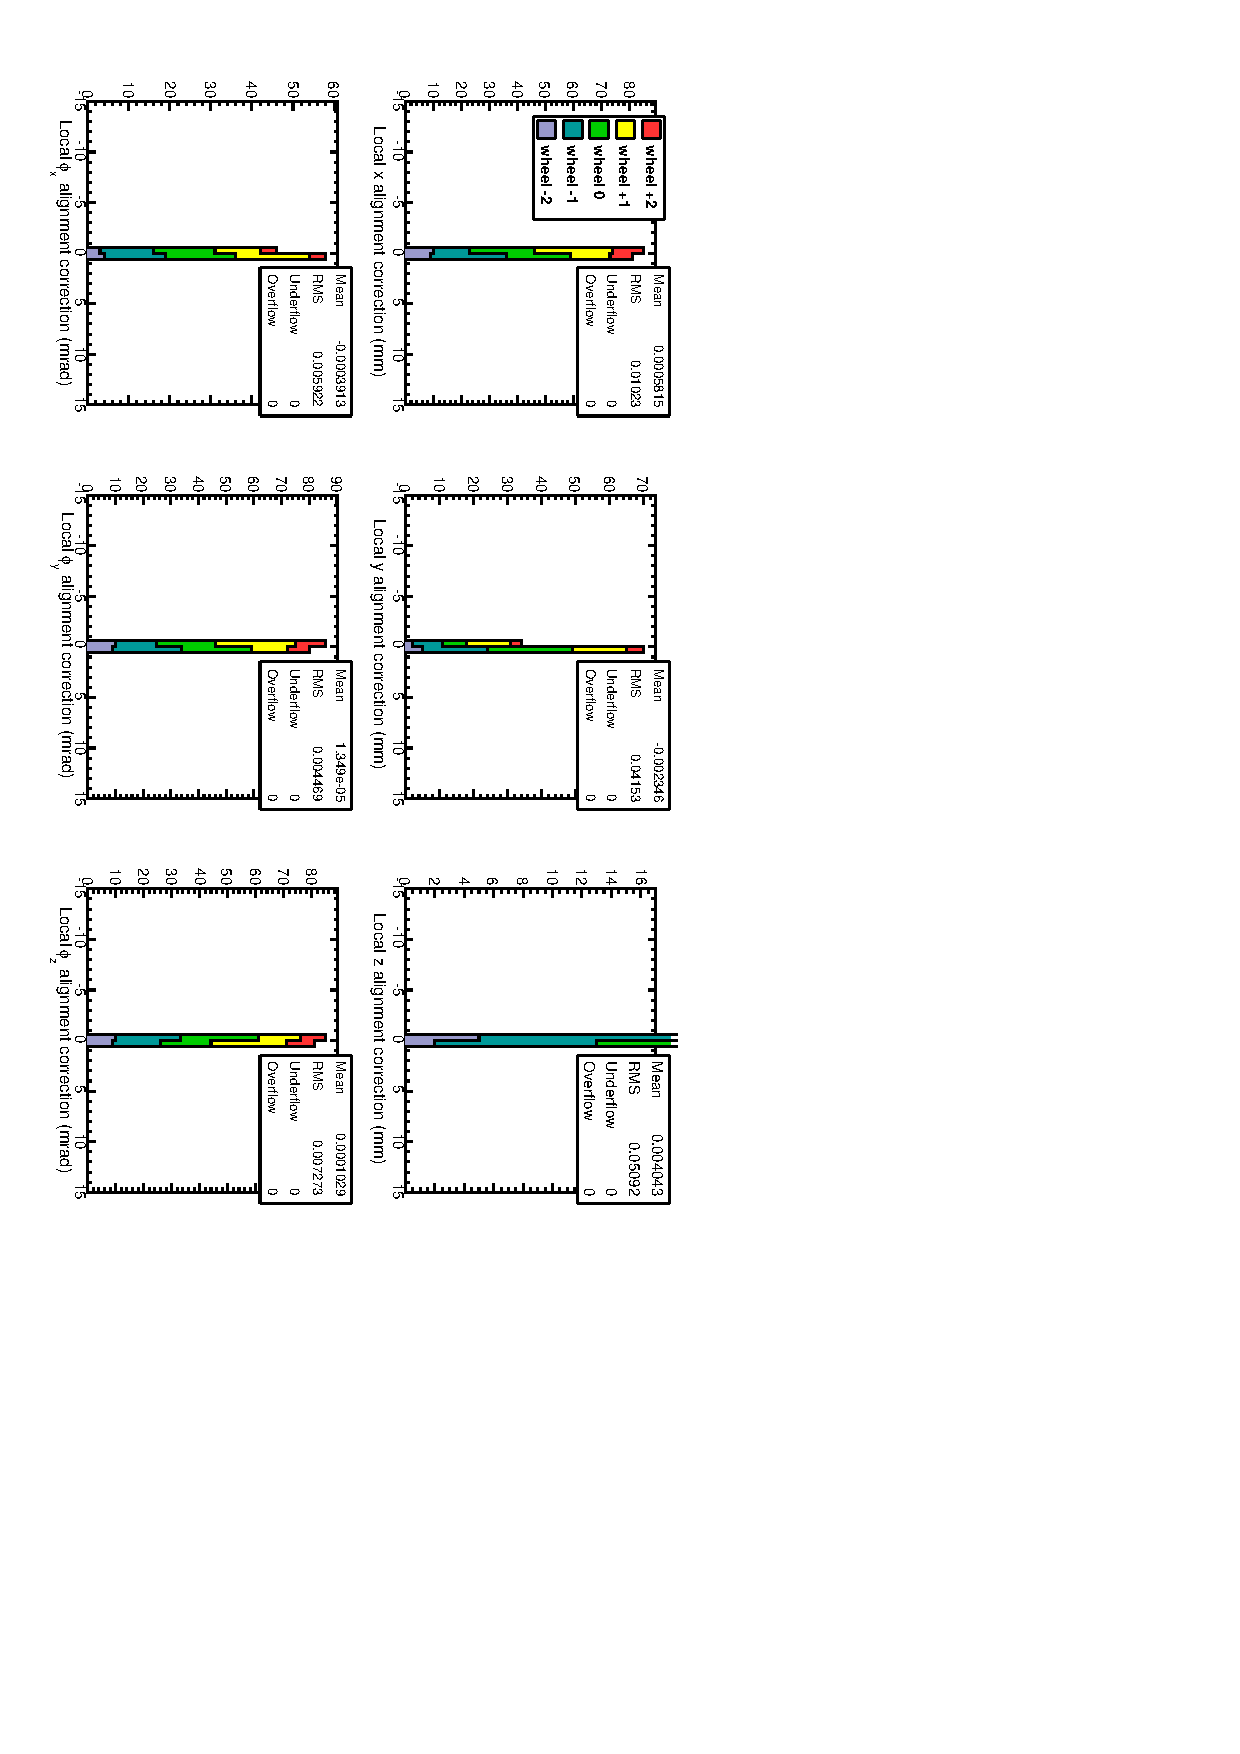
\includegraphics[height=\linewidth, angle=90]{data_100GeV_newinternal_iter5.pdf}
\end{frame}

\begin{frame}
\frametitle{Beginning-to-end changes}
\vfill
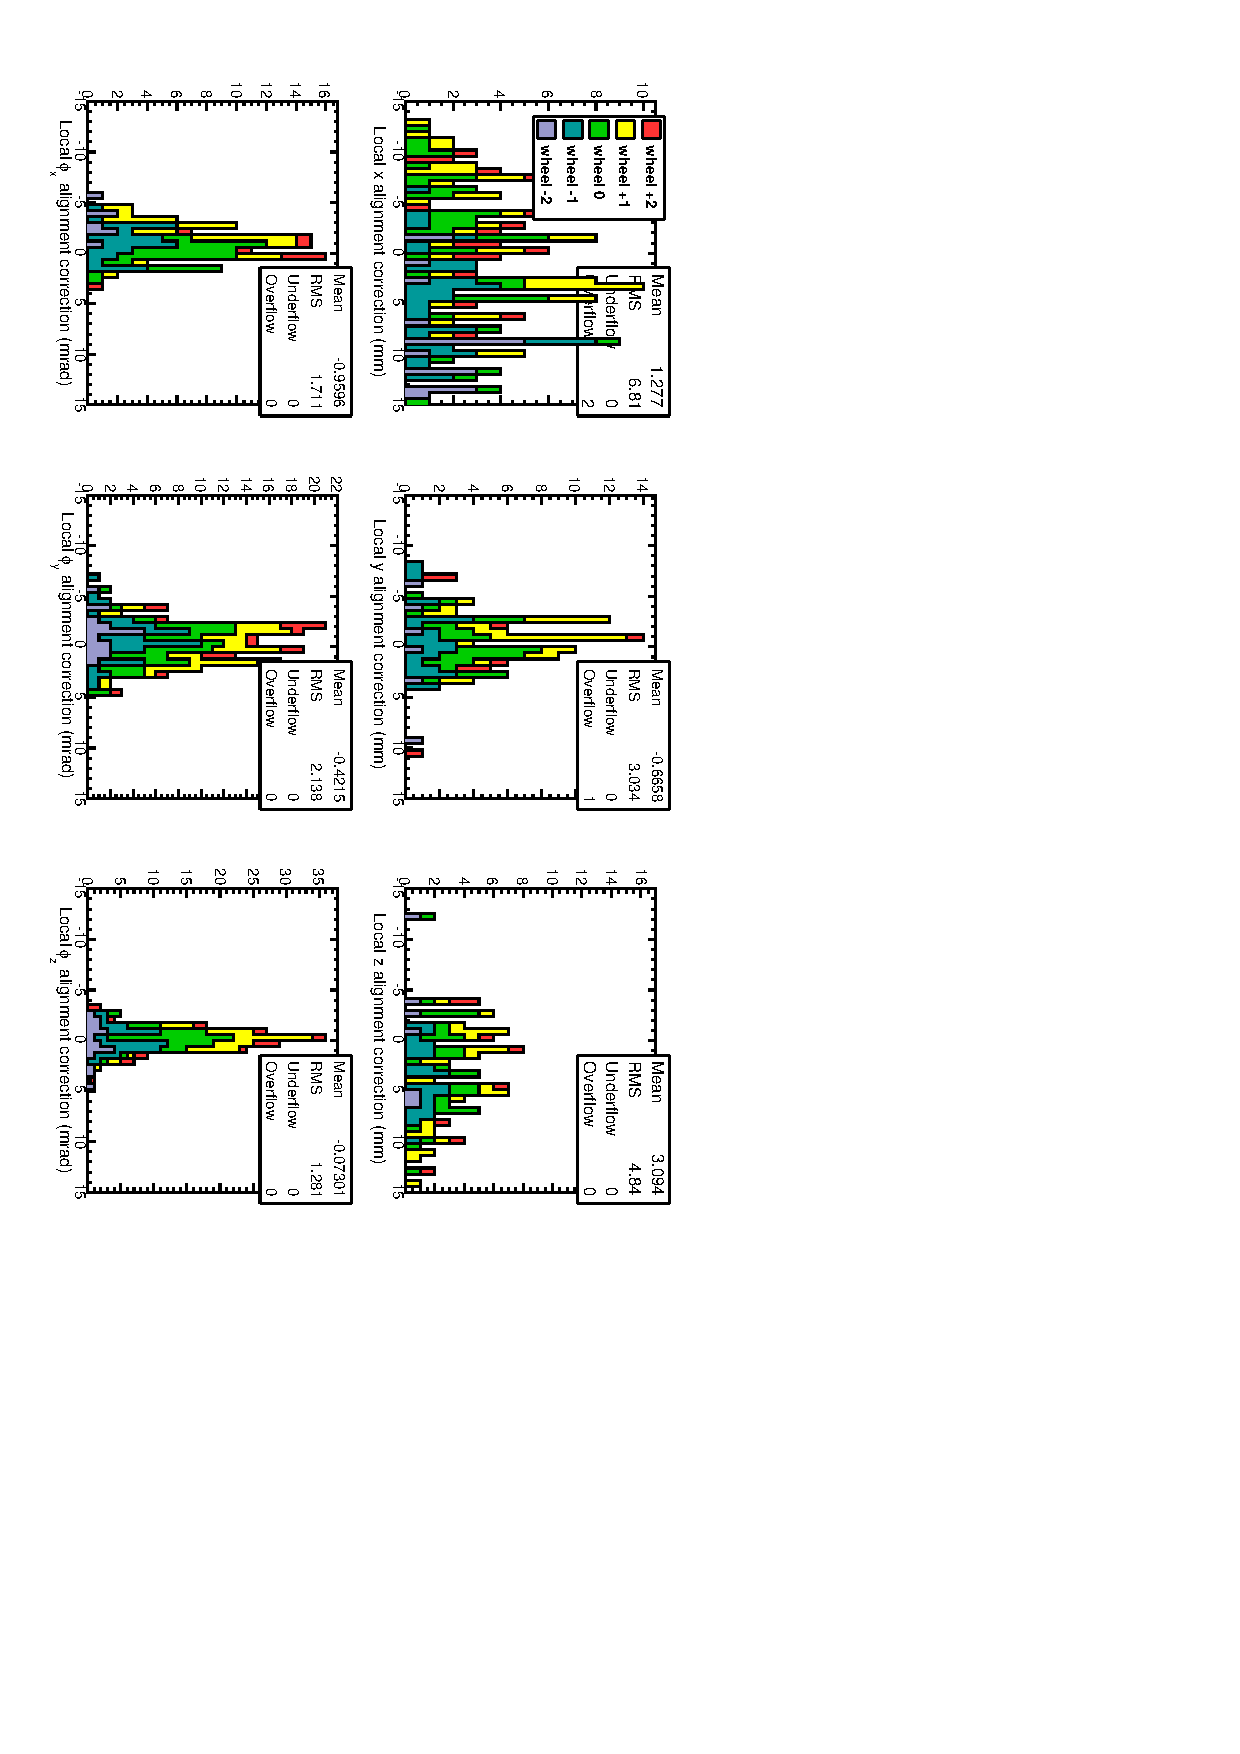
\includegraphics[height=\linewidth, angle=90]{data_100GeV_newinternal_iterall.pdf}
\end{frame}

\begin{frame}
\frametitle{Statistical uncertainties}
\vfill
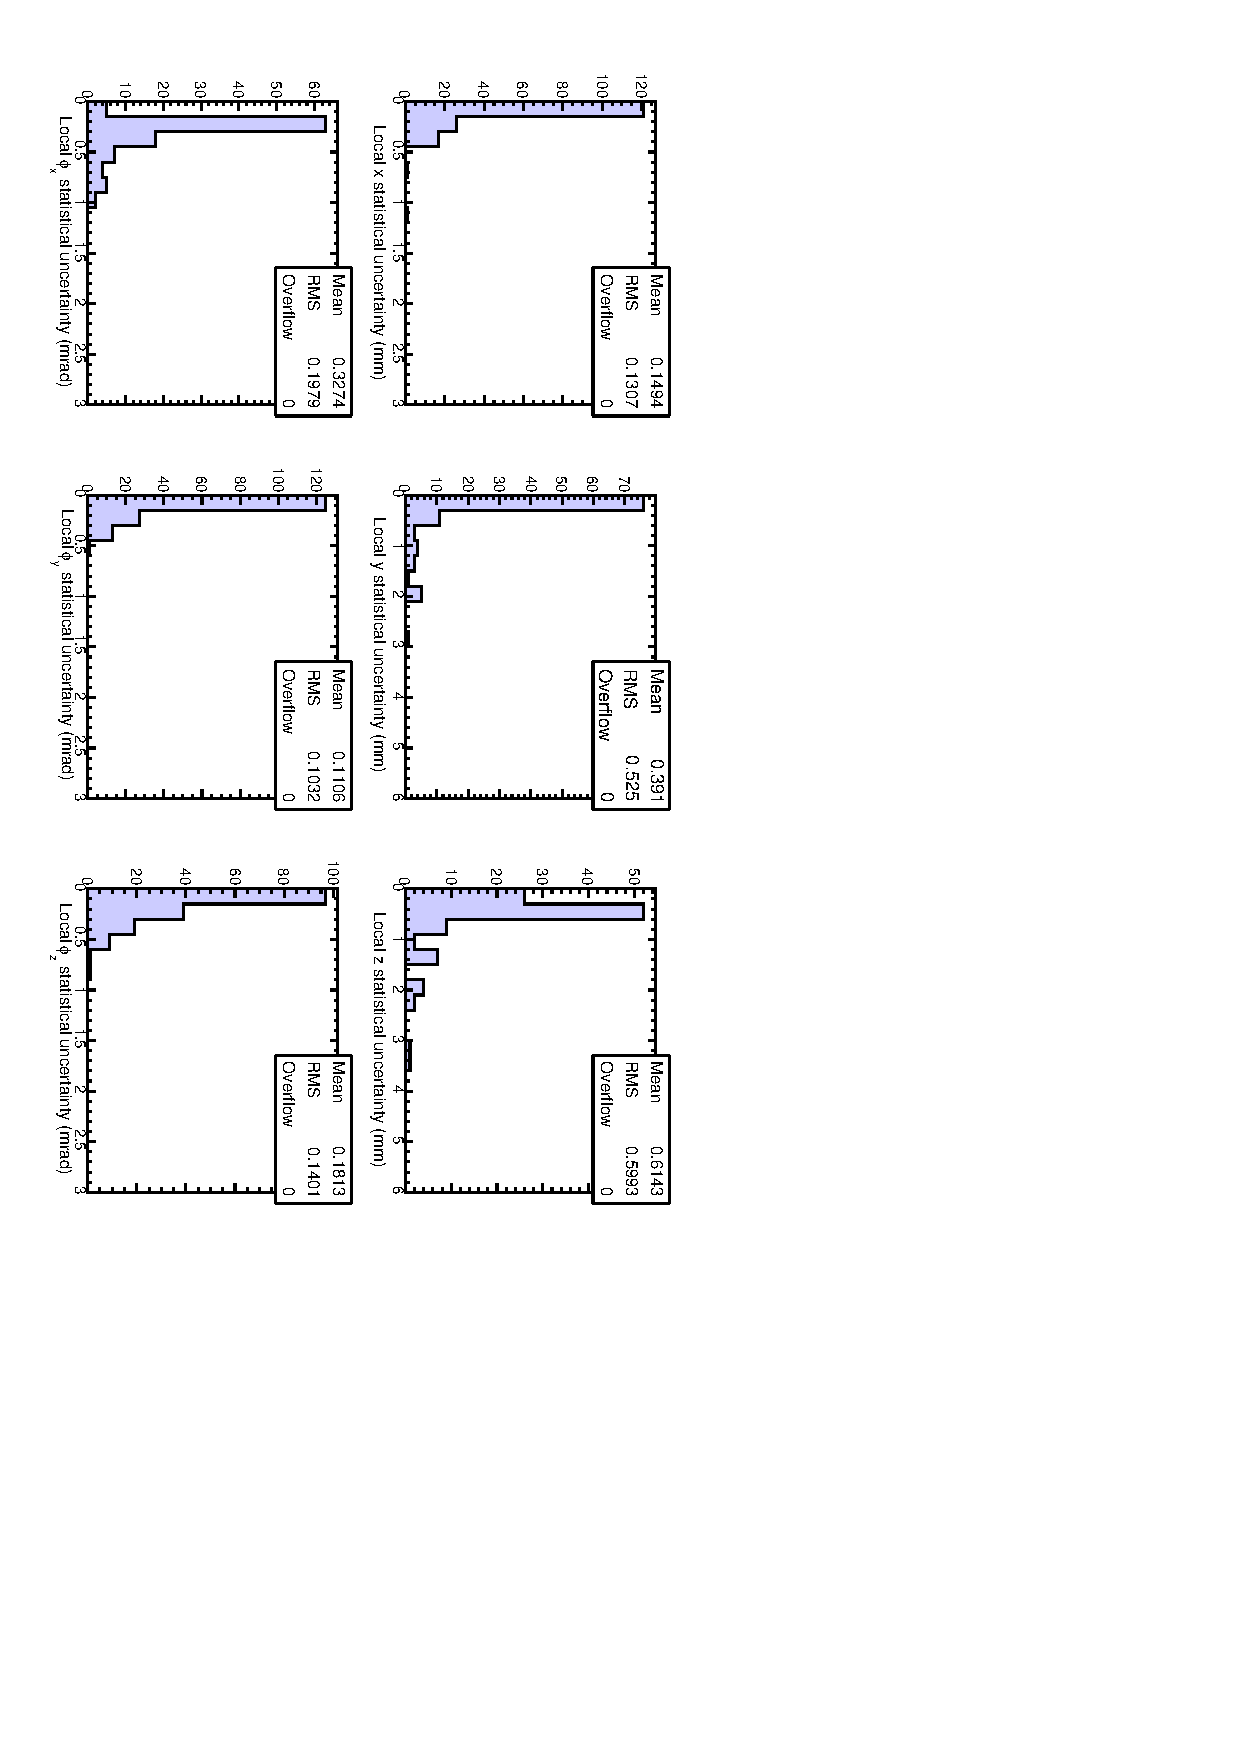
\includegraphics[height=\linewidth, angle=90]{data_100GeV_newinternal_quoted_uncertainty.pdf}
\end{frame}

\begin{frame}
\frametitle{One chamber}

\only<1>{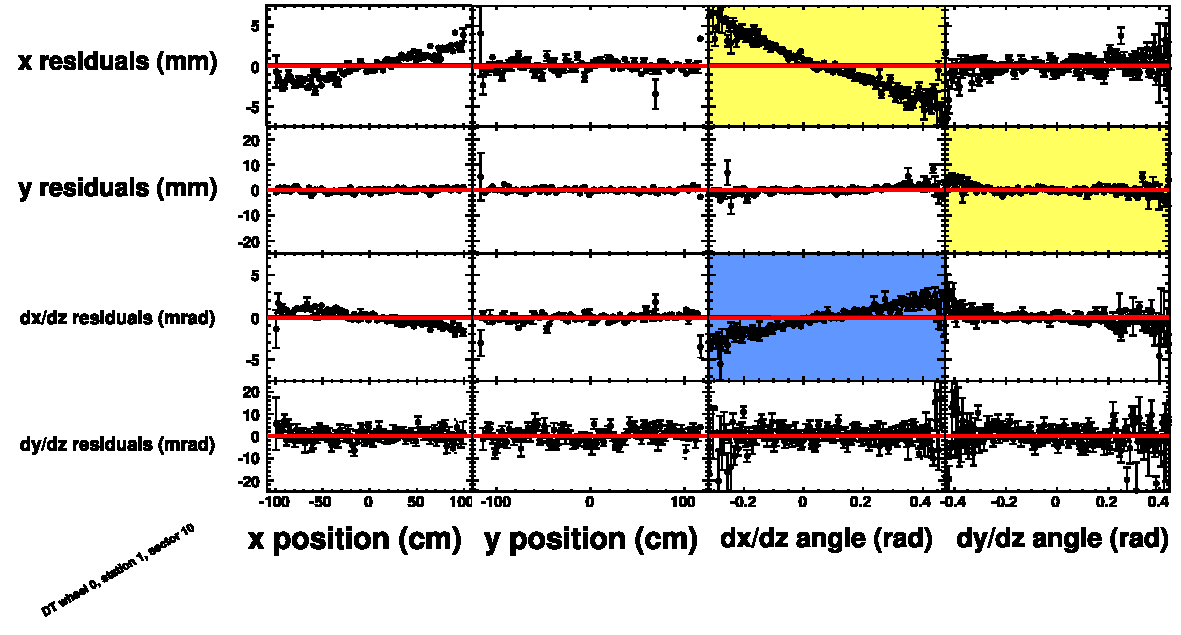
\includegraphics[width=\linewidth]{datafit_wh0st1sec10_highp.pdf}}
\only<2>{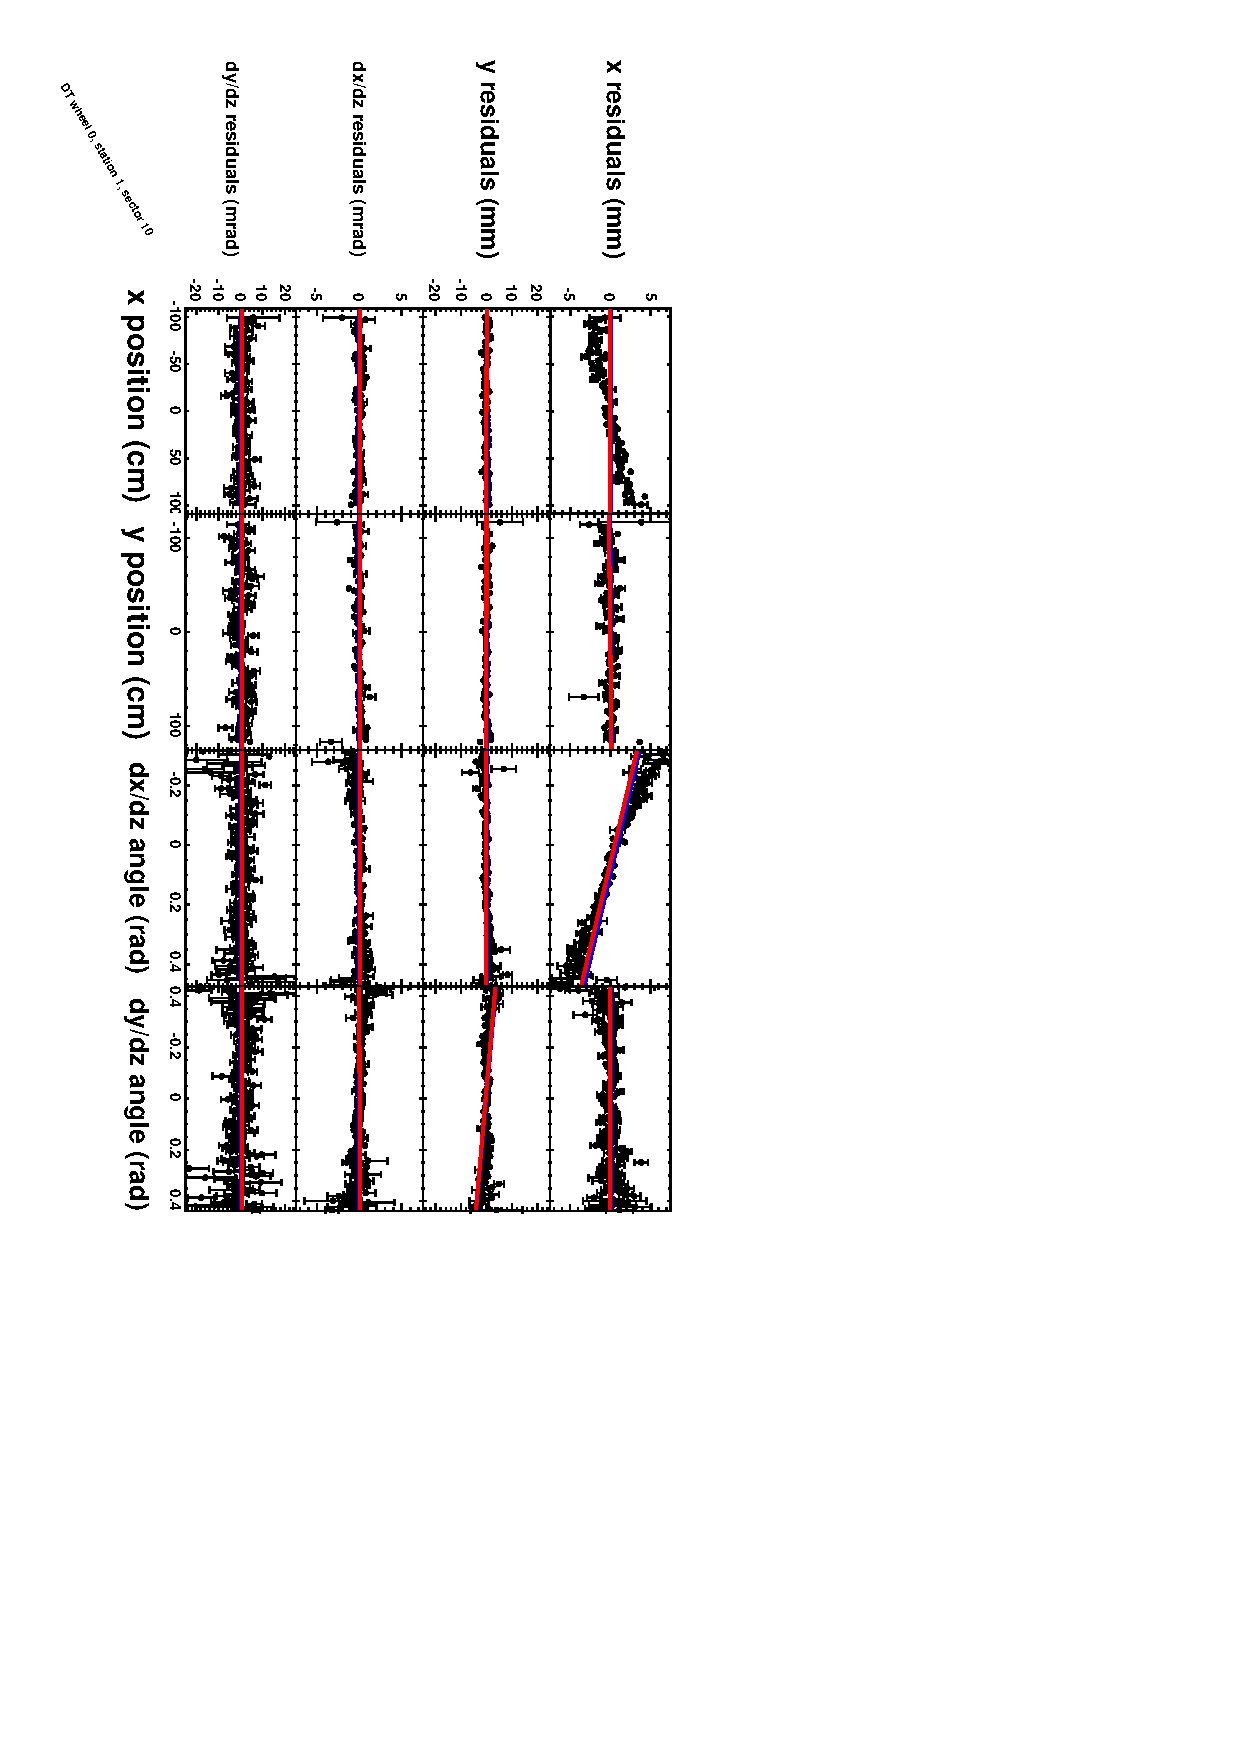
\includegraphics[height=\linewidth, angle=90]{datafit_100GeV_newinternal_whCst1sec10_iter3.pdf}}
\only<3>{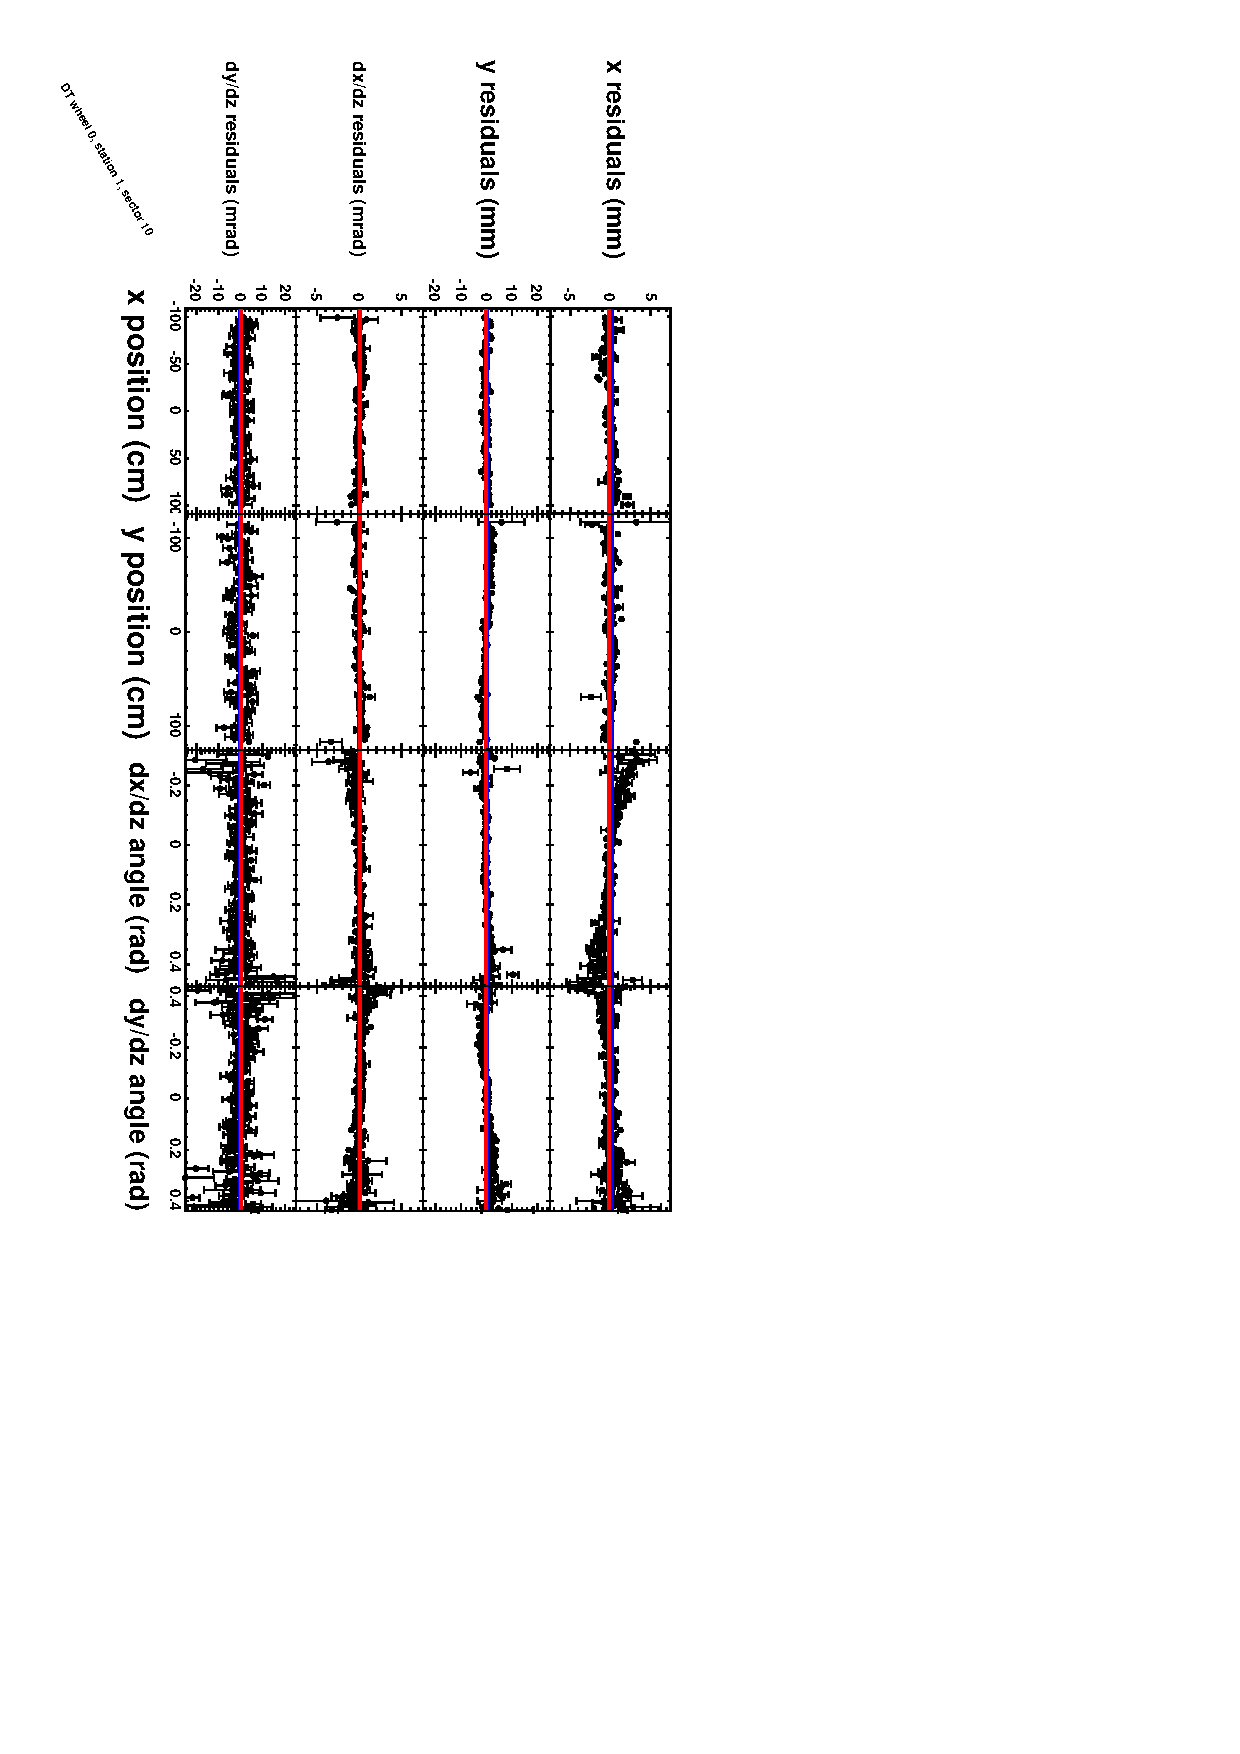
\includegraphics[height=\linewidth, angle=90]{datafit_100GeV_newinternal_whCst1sec10_iter5.pdf}}
\end{frame}

\begin{frame}
\frametitle{Sawtooth on all chambers}

\only<1>{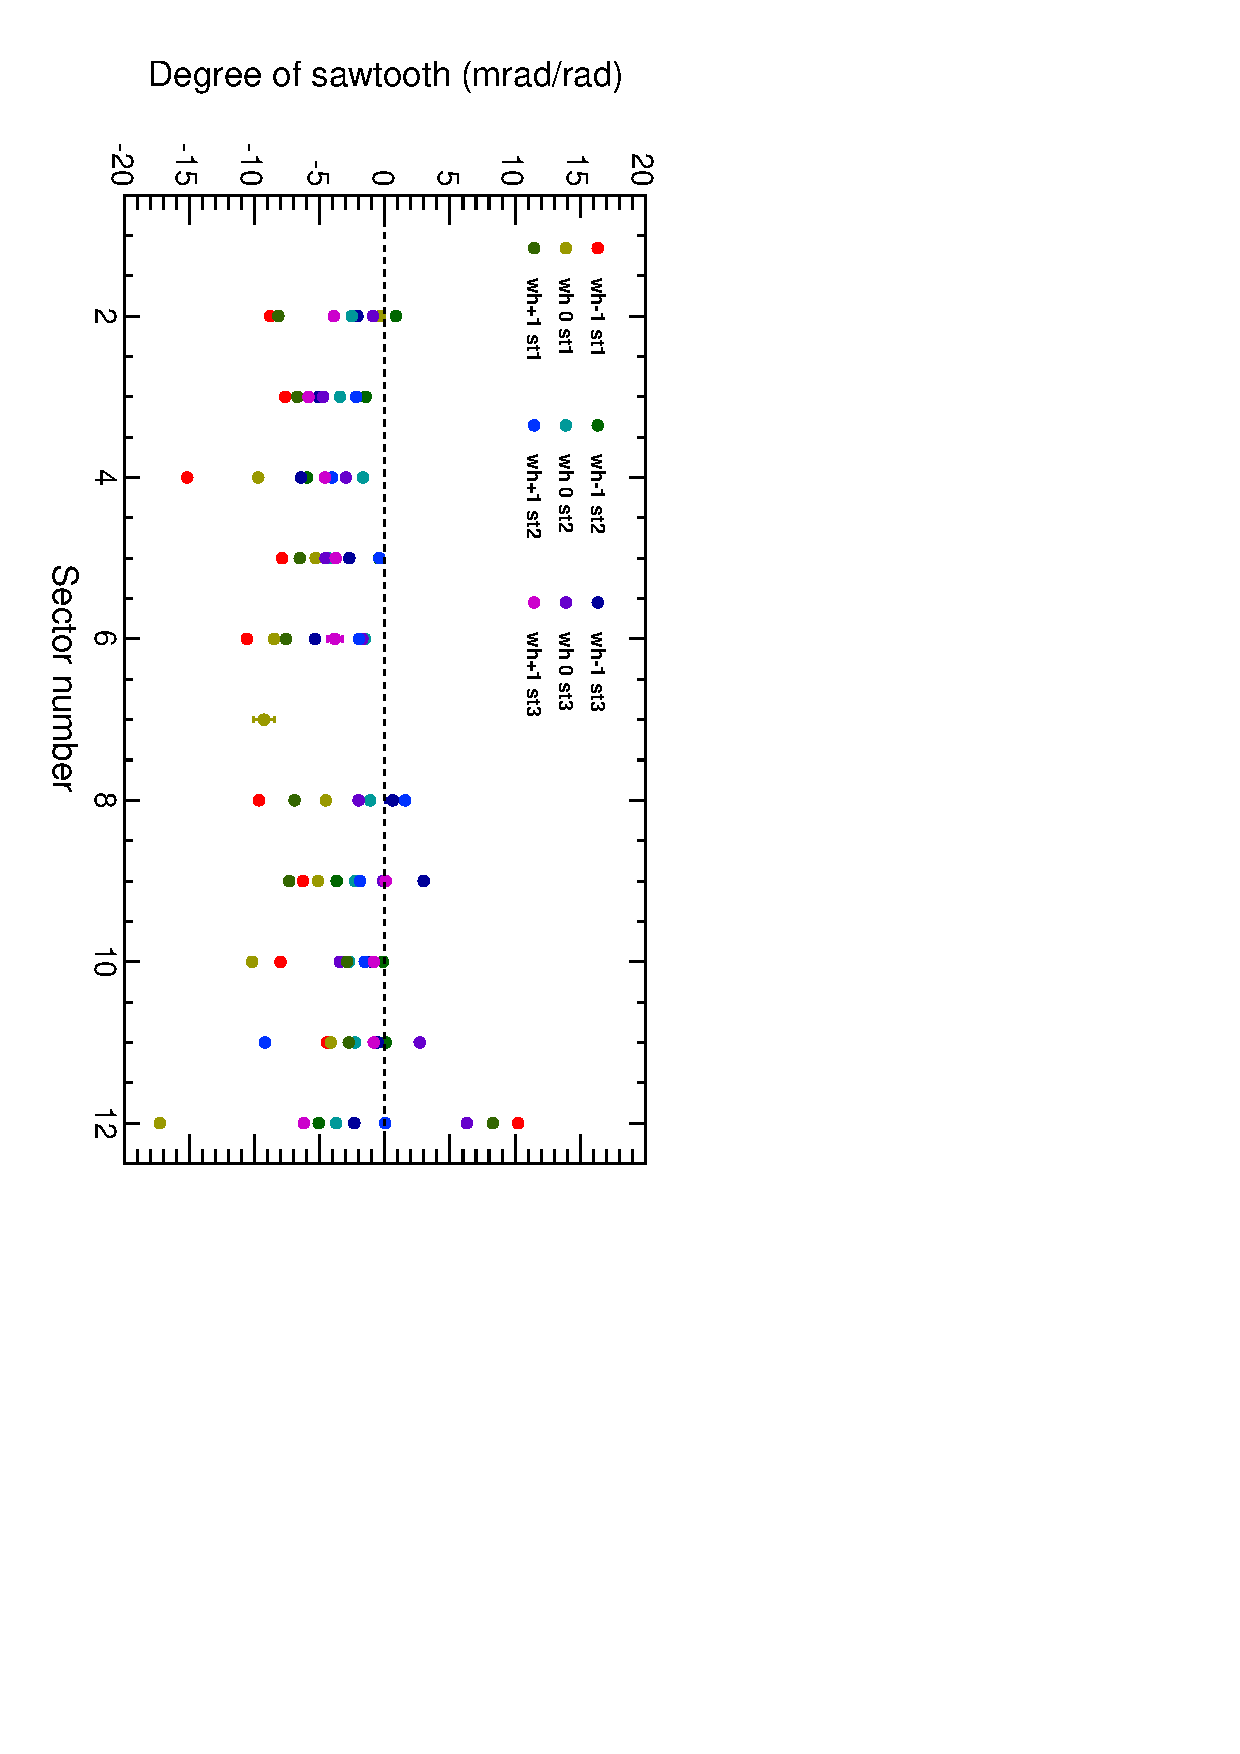
\includegraphics[height=\linewidth, angle=90]{sawtooth_bysector_lowp.pdf}}
\only<2>{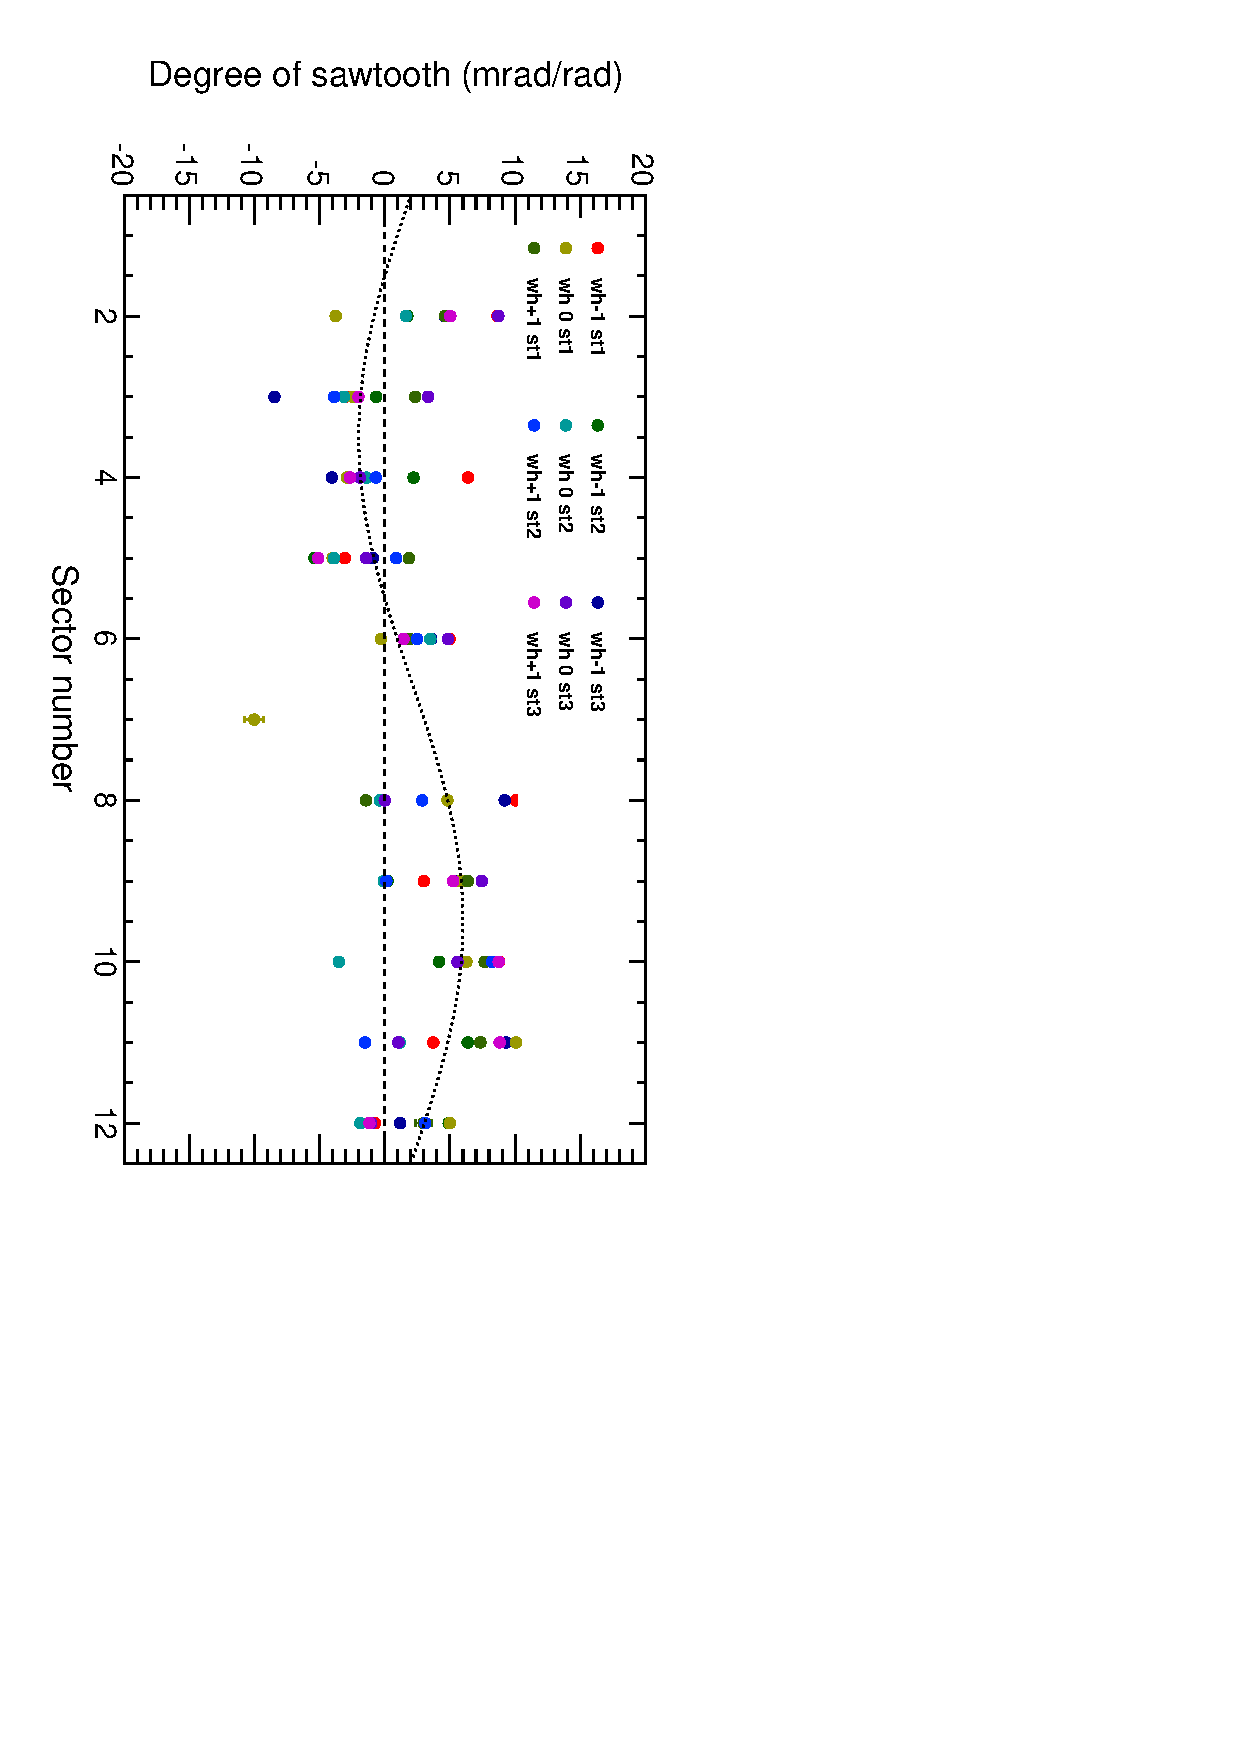
\includegraphics[height=\linewidth, angle=90]{sawtooth_bysector_highp.pdf}}
\only<3>{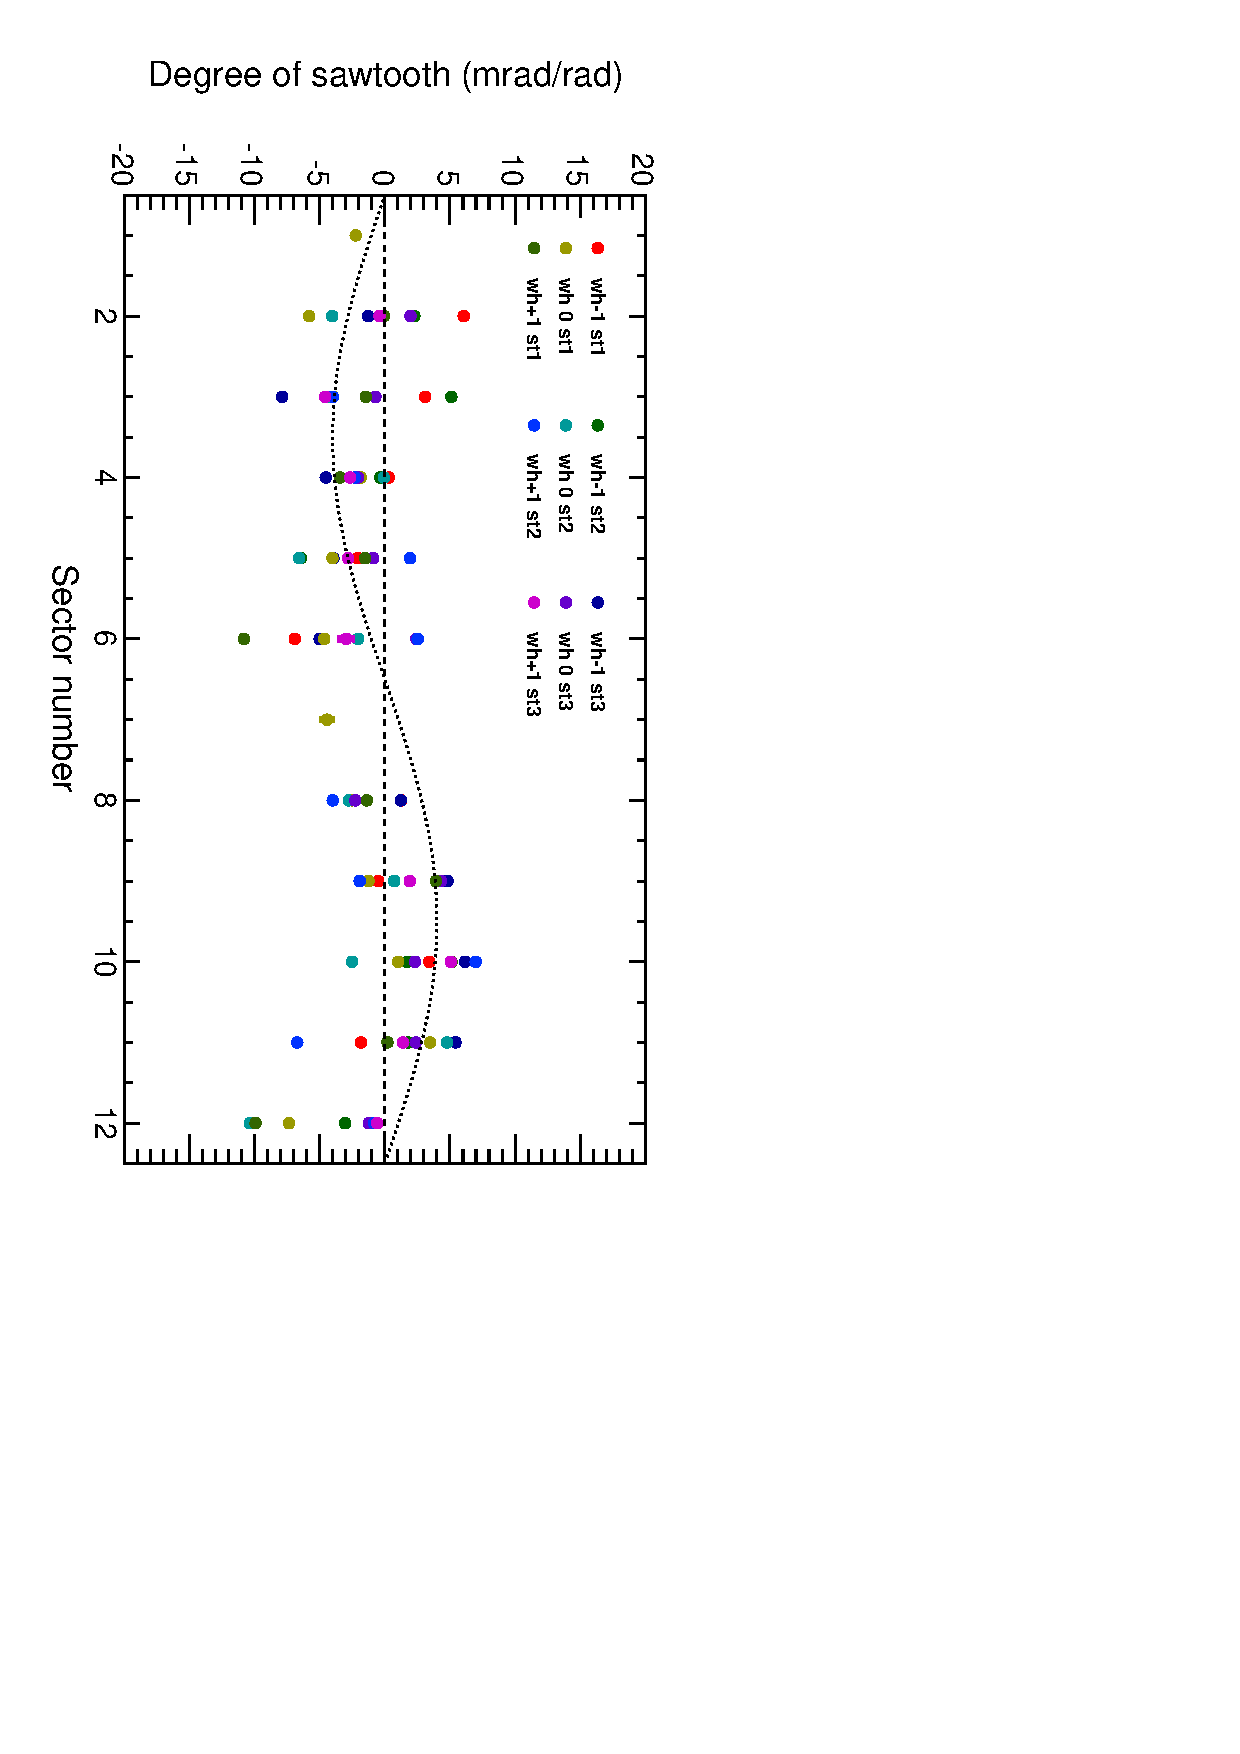
\includegraphics[height=\linewidth, angle=90]{sawtooth_bysector_highp_newinternal.pdf}}
\only<4>{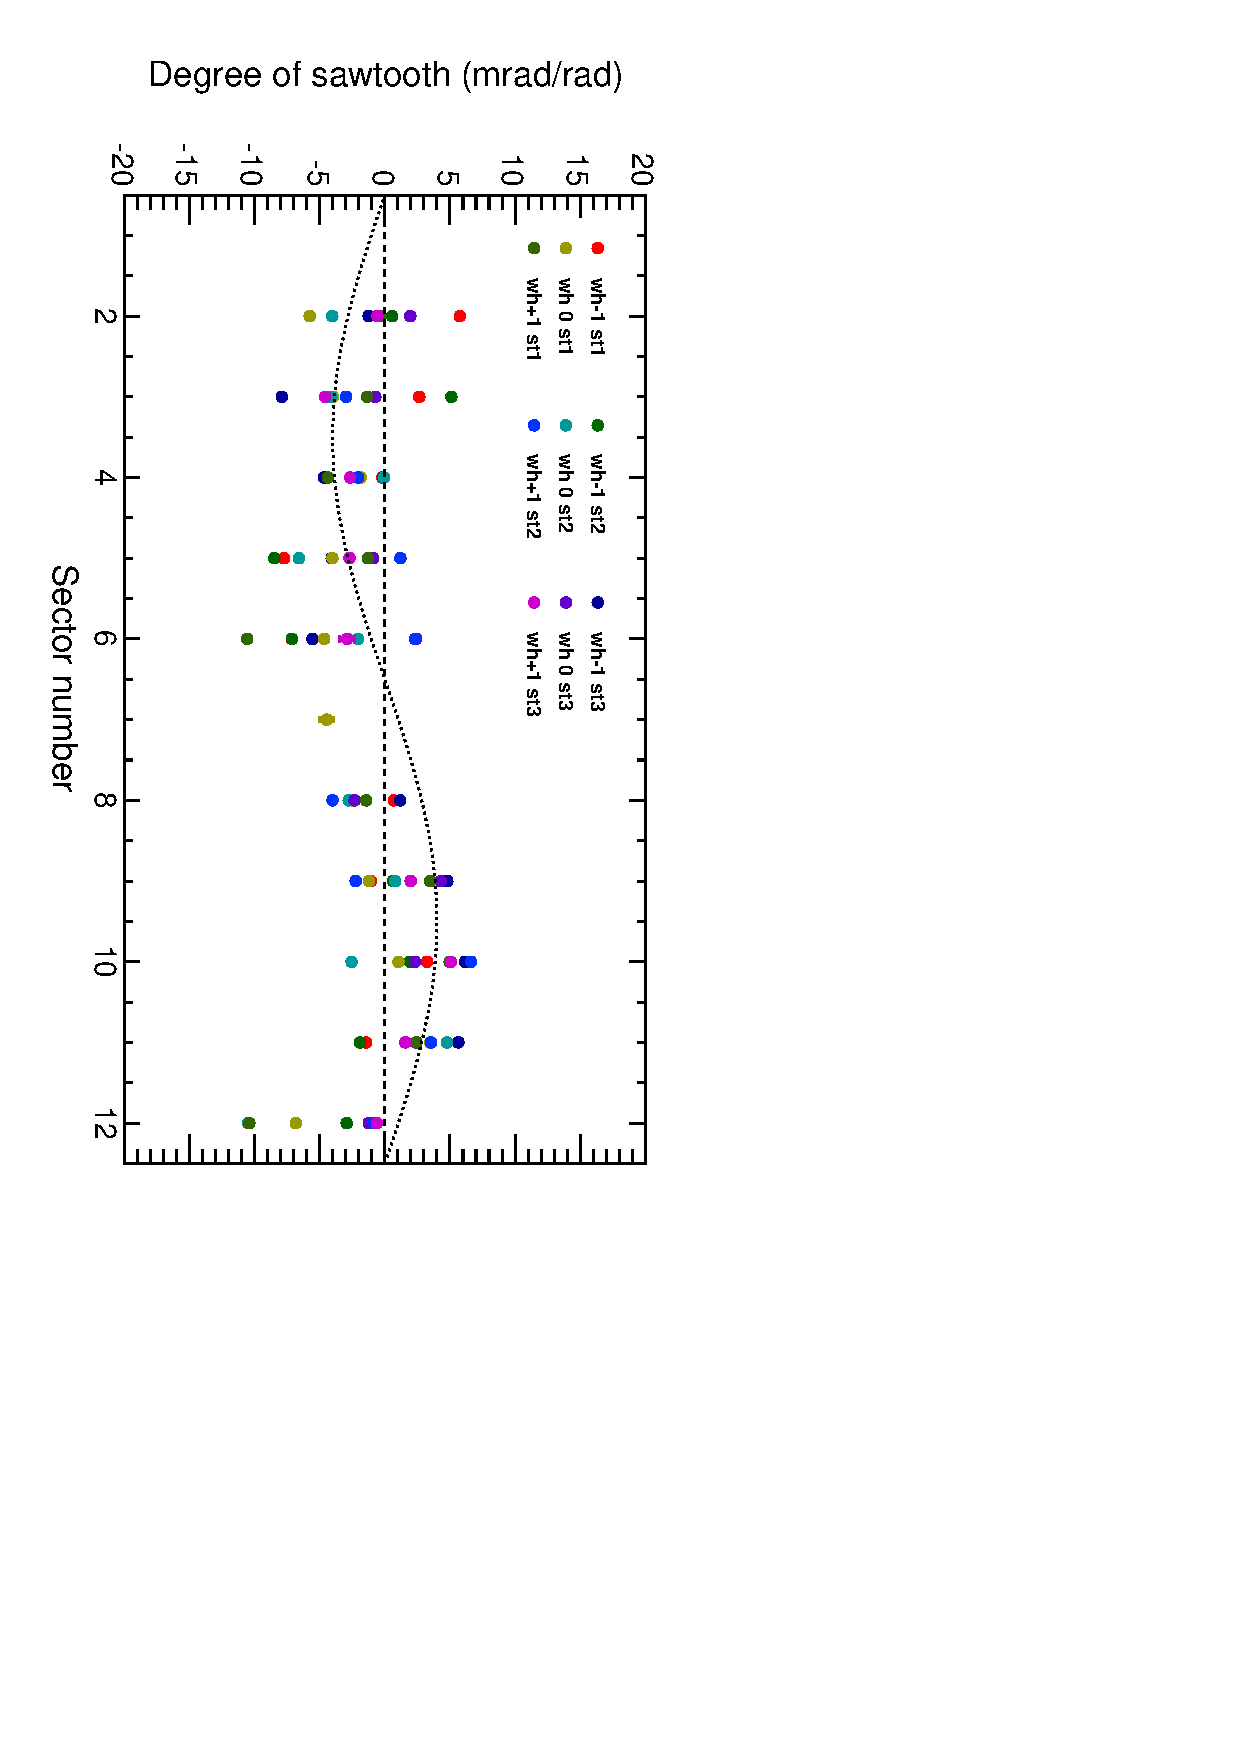
\includegraphics[height=\linewidth, angle=90]{sawtooth_bysector_highp_newinternal_zalign.pdf}}
\only<5>{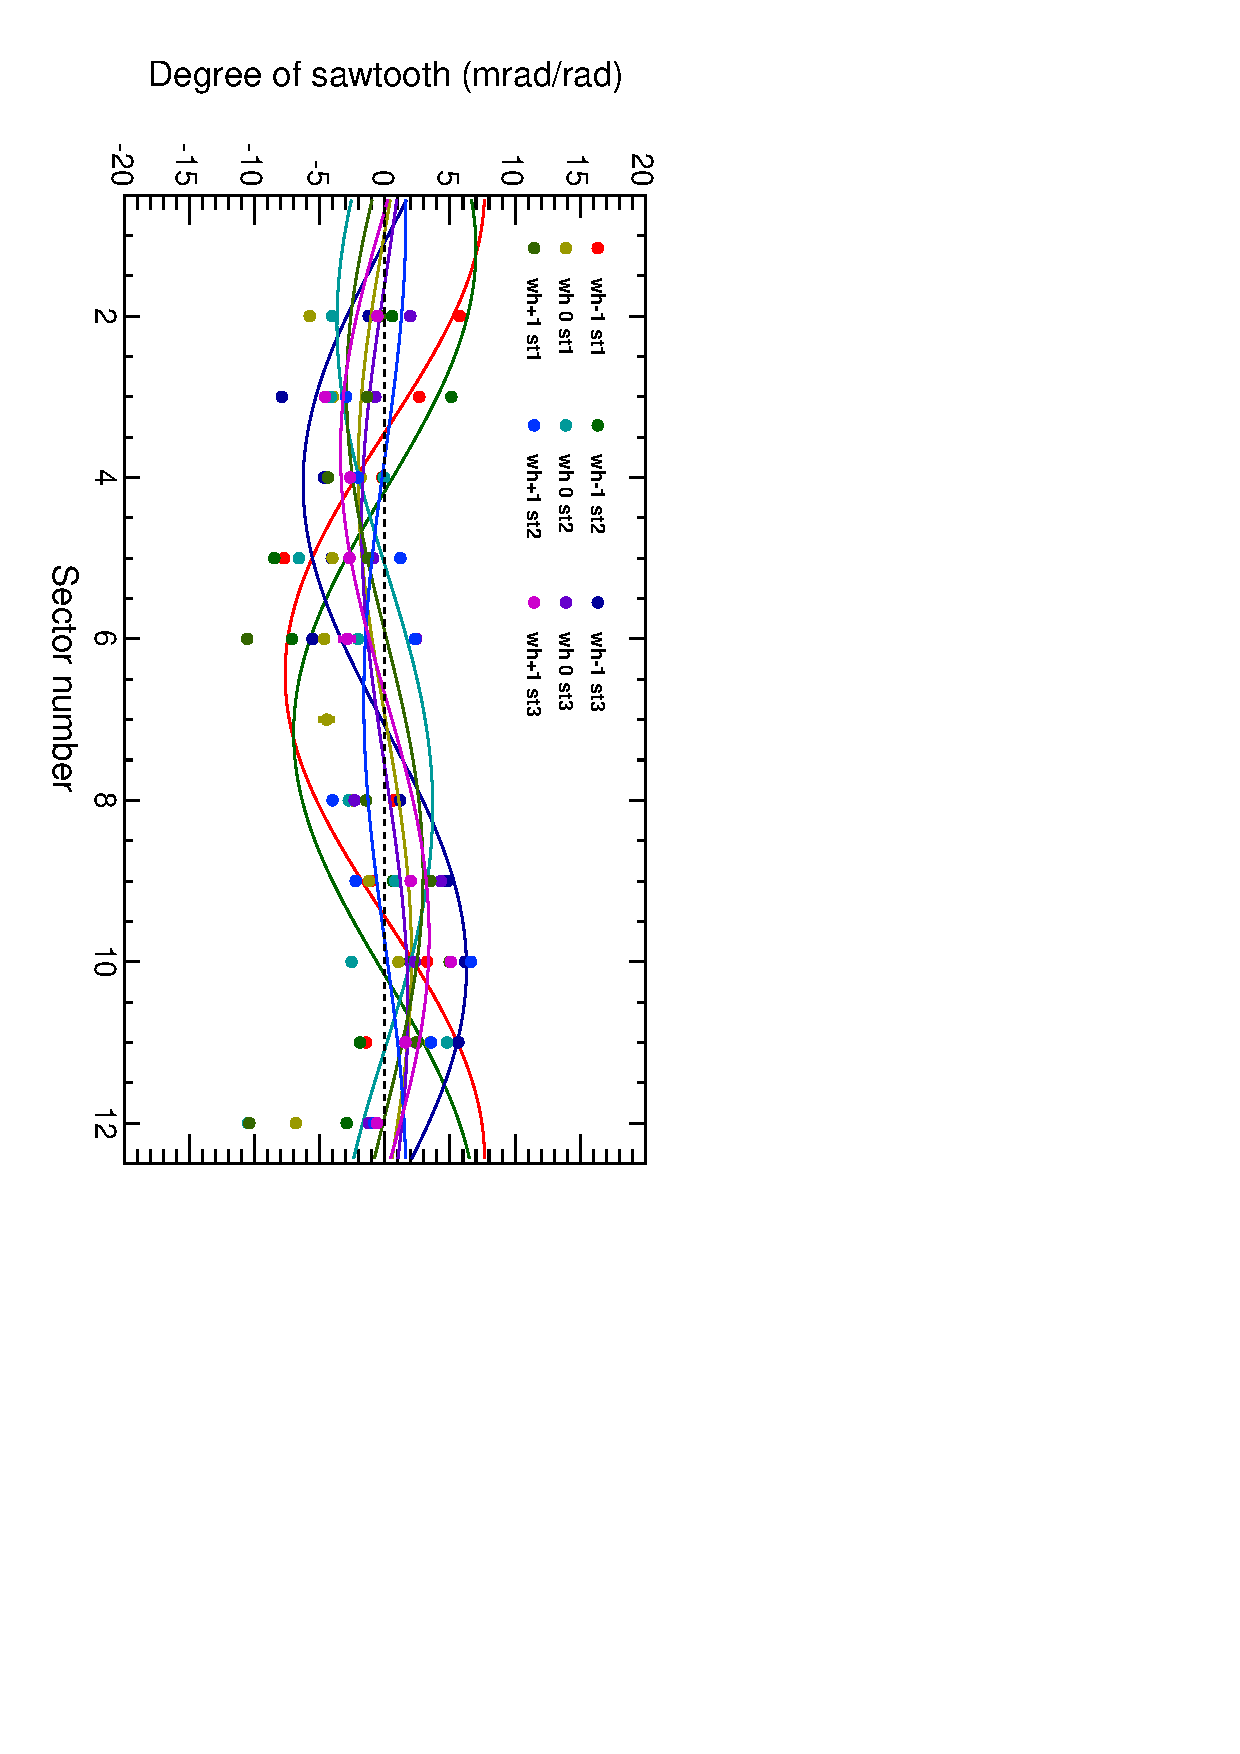
\includegraphics[height=\linewidth, angle=90]{sawtooth_bysector_highp_newinternal_zalign_fits.pdf}}
\only<6>{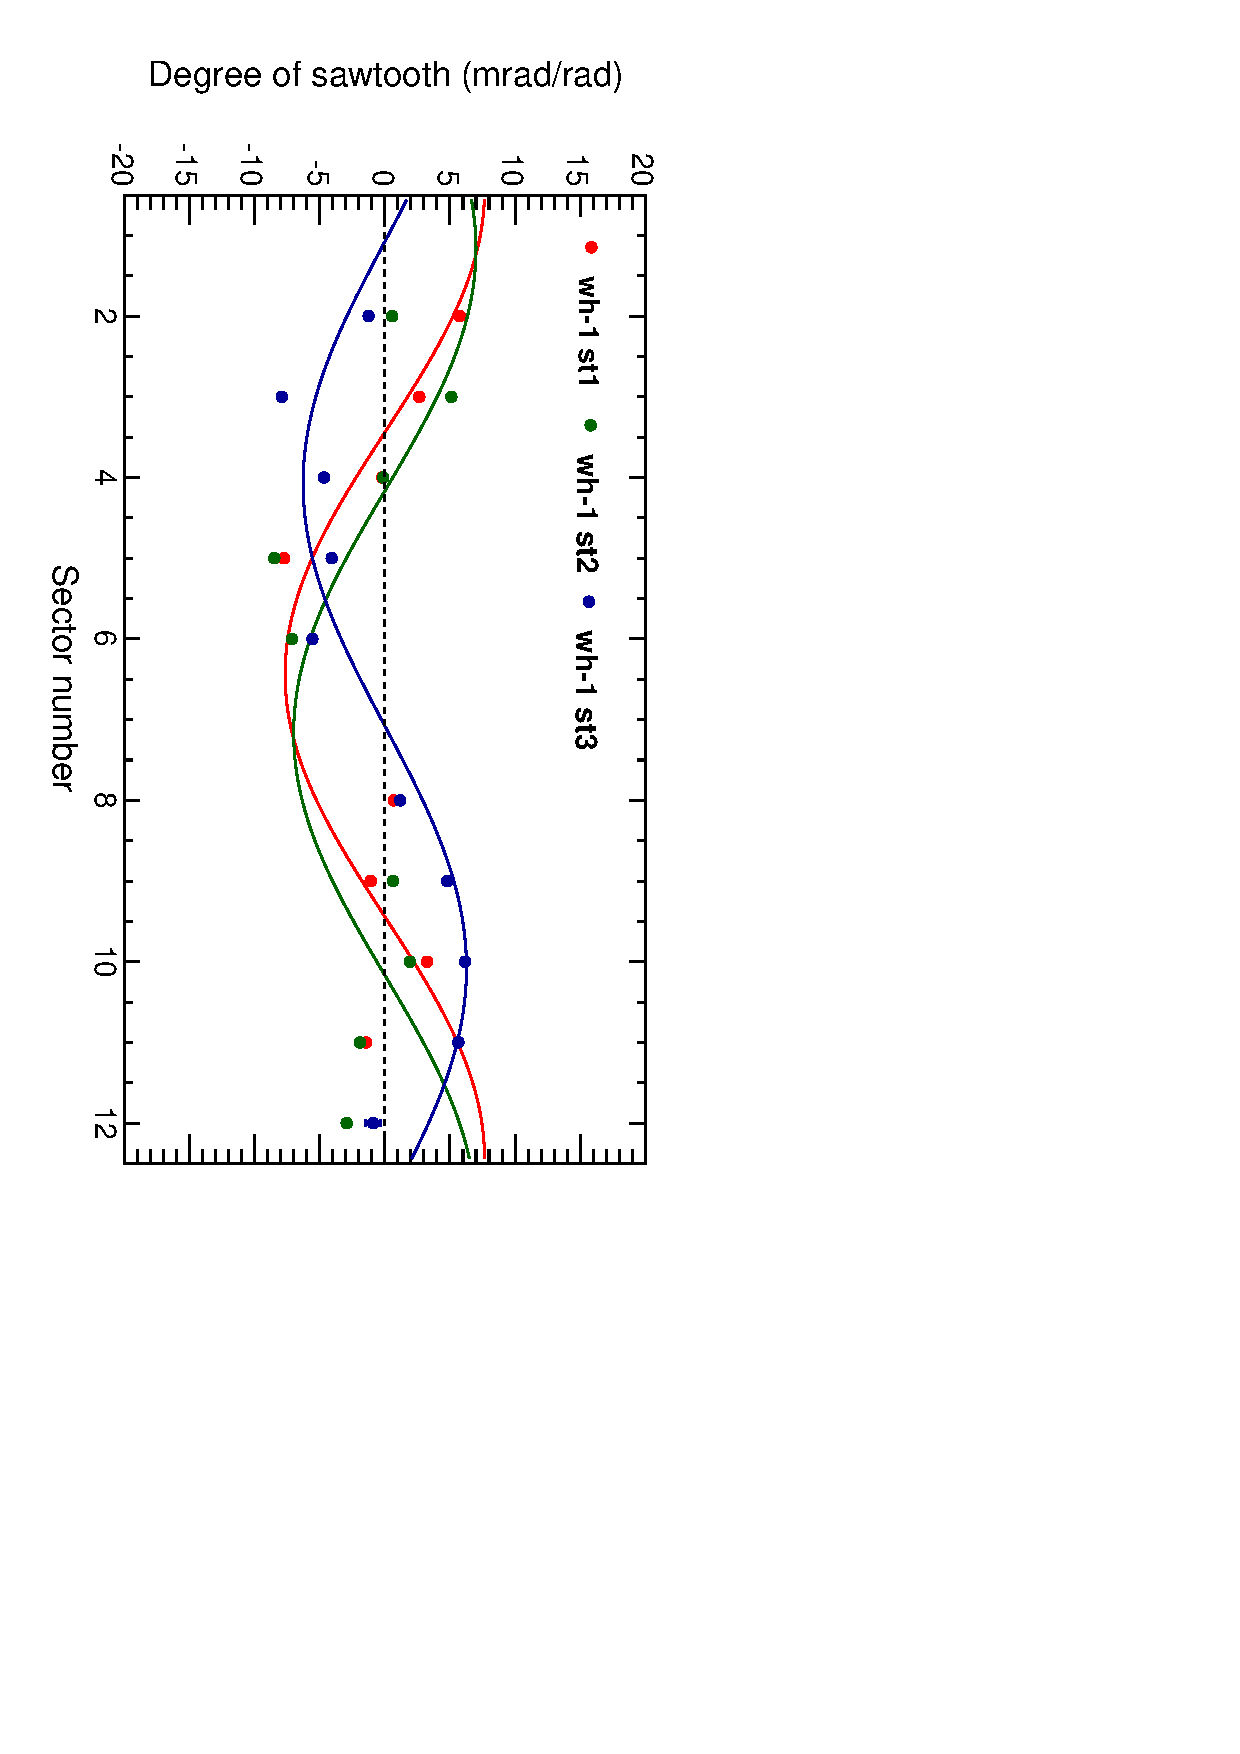
\includegraphics[height=\linewidth, angle=90]{sawtooth_bysector_highp_newinternal_zalign_fits2.pdf}}
\only<7>{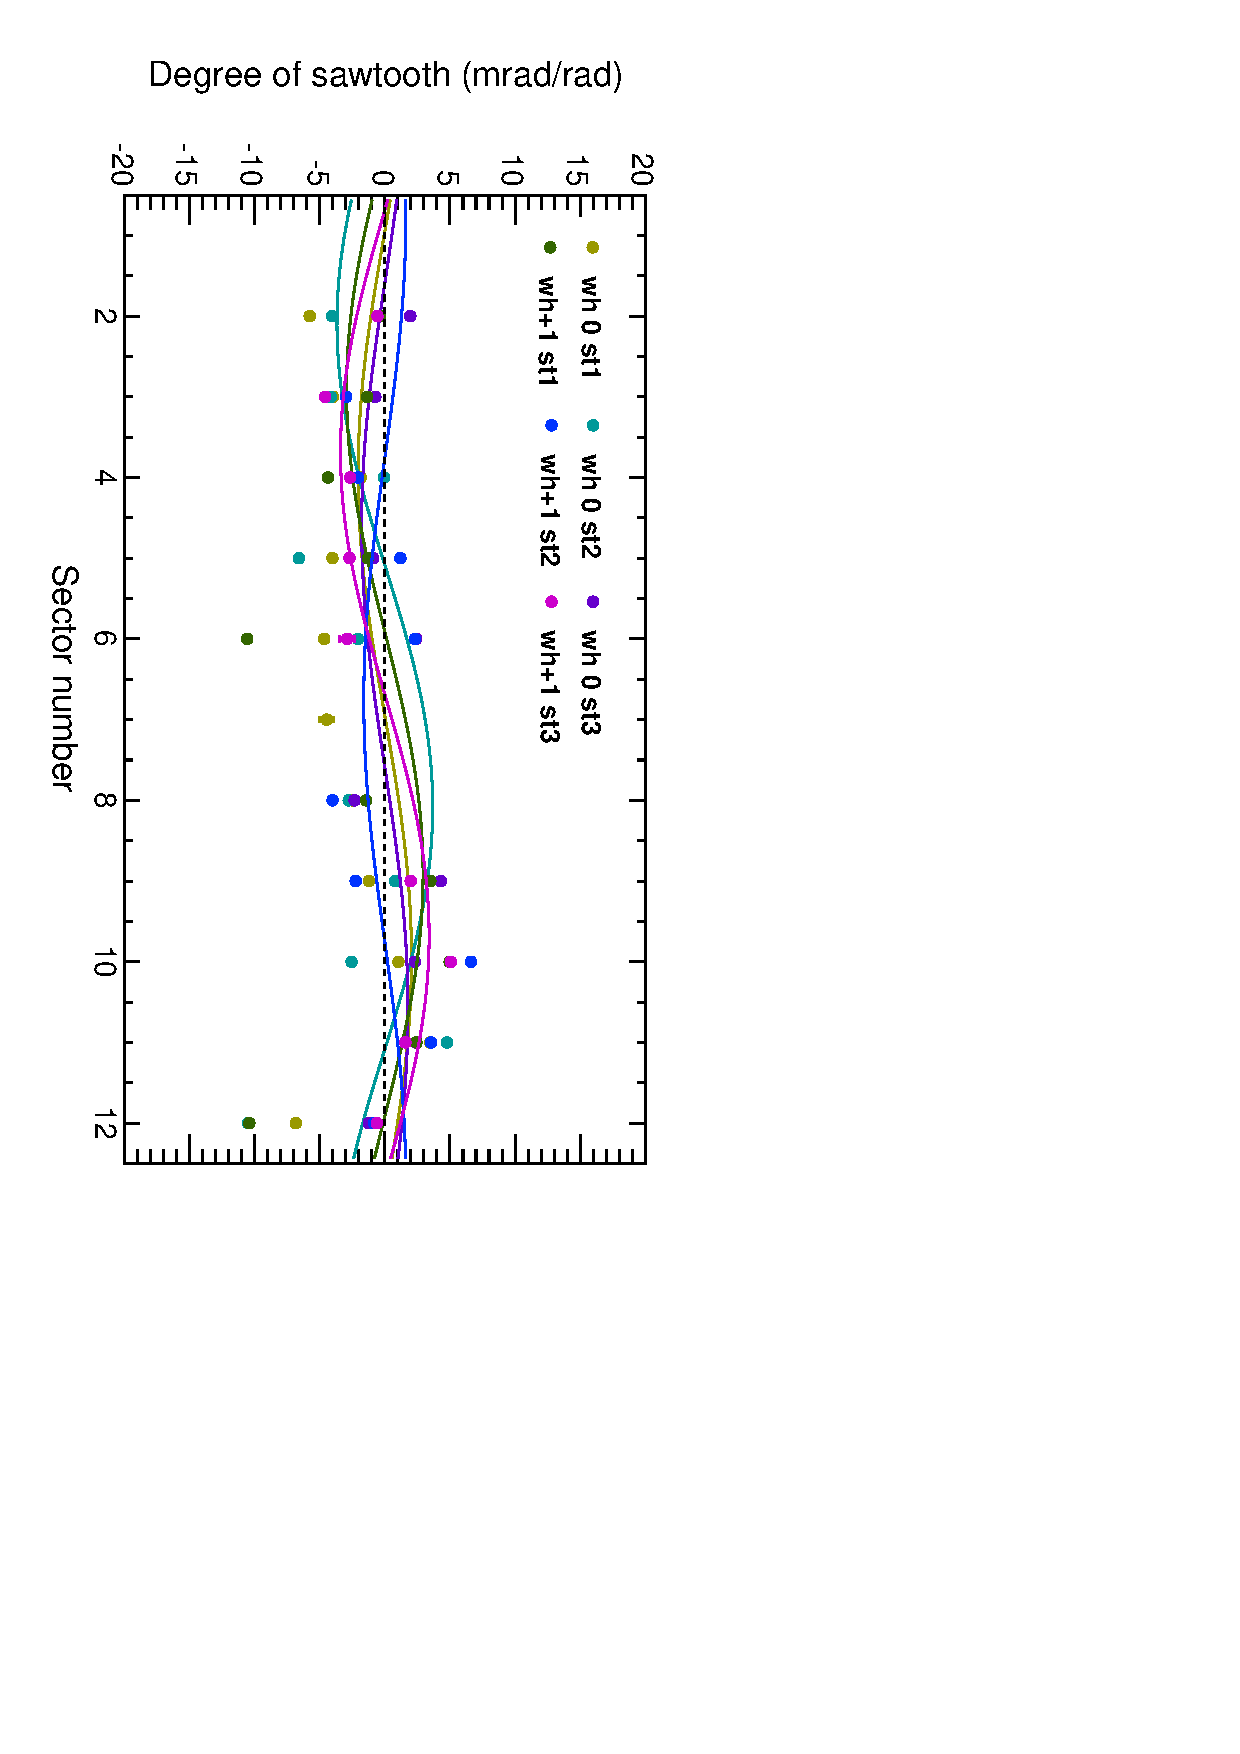
\includegraphics[height=\linewidth, angle=90]{sawtooth_bysector_highp_newinternal_zalign_fits3.pdf}}

\end{frame}

\begin{frame}
\frametitle{Conclusions}

\begin{itemize}
\item New DT alignment has an effect on sawtooth, but doesn't solve it for all chambers
\item Sawtooths are exhibiting a global pattern in addition to a chamber-by-chamber scatter
\begin{itemize}
\item the global pattern may be from the track source
\end{itemize}

\item Big improvement in tracker alignment is coming (their mean
  $\chi^2$ is about 1.4 now, even without APEs), we need to use that
  in our next signed-off constants

\item This (including the tracker input) is the DT alignment that I'll
  use to align the endcap

\end{itemize}
\label{numpages}

\end{frame}







%% \begin{frame}
%% \frametitle{Outline}
%% \begin{itemize}\setlength{\itemsep}{0.75 cm}
%% \item 
%% \end{itemize}
%% %% \hspace{-0.83 cm} \textcolor{darkblue}{\Large Outline2}
%% \end{frame}

%% \section*{First section}
%% \begin{frame}
%% \begin{center}
%% \Huge \textcolor{blue}{First section}
%% \end{center}
%% \end{frame}

%% \begin{frame}
%% \end{frame}

\end{document}
